\documentclass[a4paper, 10pt]{article}
%\usepackage[utf8]{inputenc}			
\usepackage[ngerman]{babel}		% for german	
\usepackage{graphicx}
\usepackage{psfrag}								
\usepackage{parskip}
\usepackage{listings}
\usepackage{xcolor}
\usepackage{amsmath}
\usepackage{mathtools}
\usepackage{amssymb}
\usepackage{mathrsfs}
\usepackage{empheq}
\usepackage{titlesec}	
\usepackage{tikz}
\usetikzlibrary{arrows}
%\usepackage{tabularx}
%\usepackage{pdfpages}
%\usepackage{hyperref,breakurl}
%\usepackage{url}
%\usepackage{psfrag}
\usepackage{epstopdf}
\usepackage{dsfont}
\usepackage{sectsty}
\allsectionsfont{\bfseries\sffamily}

\addtolength{\textwidth}{2.1cm}
\addtolength{\topmargin}{-1.4cm}
\addtolength{\oddsidemargin}{-1.1 cm}
\definecolor{leichtgrau}{gray}{0.91}
\setlength{\parindent}{0pt}

% \lstset{language = C,
	% basicstyle=\footnotesize,       
	% numbers=left,                  
	% numberstyle=\footnotesize,      
	% stepnumber=2,
	% numbersep=5pt,
	% backgroundcolor=\color{leichtgrau},
	% frame=single,
% }

% Definition von römischen Zahlen
\makeatletter
\newcommand{\rmnum}[1]{\romannumeral #1}
\newcommand{\Rmnum}[1]{\expandafter\@slowromancap\romannumeral #1@}
\makeatother
%\renewcommand{\familydefault}{\sfdefault}
\title{MIMO Skript\,-\,Wintersemester 2013 \\ Kapitel 2}
\date{}

\begin{document}
\maketitle
\tableofcontents
\setcounter{section}{1}
\section{Point\,-\,to\,-\,Point MIMO Systems}
\subsection{MIMO Channel Capacity}
Inhalt: s. Skript in VL ausgeteilt
\subsection{SIMO Systems}
\paragraph{Remarks}
\begin{itemize}
	\item In SIMO Systems only \underline{coding} and \underline{diversity} \underline{gains} can be exploited (no multiplexing gains)
	\item To realize these gains diversity combining has to be performed
	\item Diversity combining schemes vary in complexity and performance
	\item There are \underline{many} diversity combining schemes. Here we consider:
	\begin{itemize}
		\item Maximal ratio combining (MRC)
		\item Equal gain combining (EGC)
		\item Selection combining (SC)
	\end{itemize}
	\item Diversity combining problem
	\begin{figure}[ht]
		\centering
		\psfrag{h_1}[hl][hl]{$h_1$}
		\psfrag{n_1}[hl][hl]{$n_1$}
		\psfrag{w_1}[hl][hl]{$h_1$}
		\psfrag{h_NR}[hl][hl]{$h_{N_R}$}
		\psfrag{n_NR}[hl][hl]{$n_{N_R}$}
		\psfrag{w_NR}[hl][hl]{$w_{N_R}$}
		\psfrag{x_dach}[hl][hl]{$\hat{x}$}
		\psfrag{x}[hl][hl]{$x$}		
		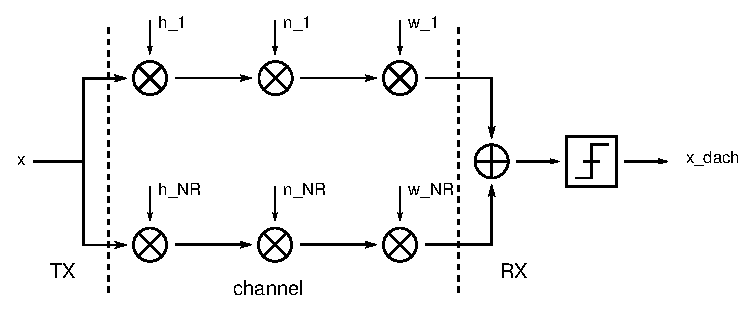
\includegraphics[width=0.8\textwidth]{Multi_Channel}
		\caption{Block Diagramm for SIMO}
		\label{fig:Multi_Channel}	
	\end{figure}		
	
	\begin{itemize}
		\item how to choose combining weights $w_n$?
		\item what performance (e.g. error rate, outage probability) is achieved?
		\item what \underline{diversity} and coding/combining gain is achieved?
	\end{itemize}
\end{itemize}

\begin{figure}
\begin{minipage}[hbt]{7cm}
	
		\centering
		\psfrag{GC_SNR_GD}[hl][hl]{$(G_c\cdot\text{SNR})^{-G_d}$}
		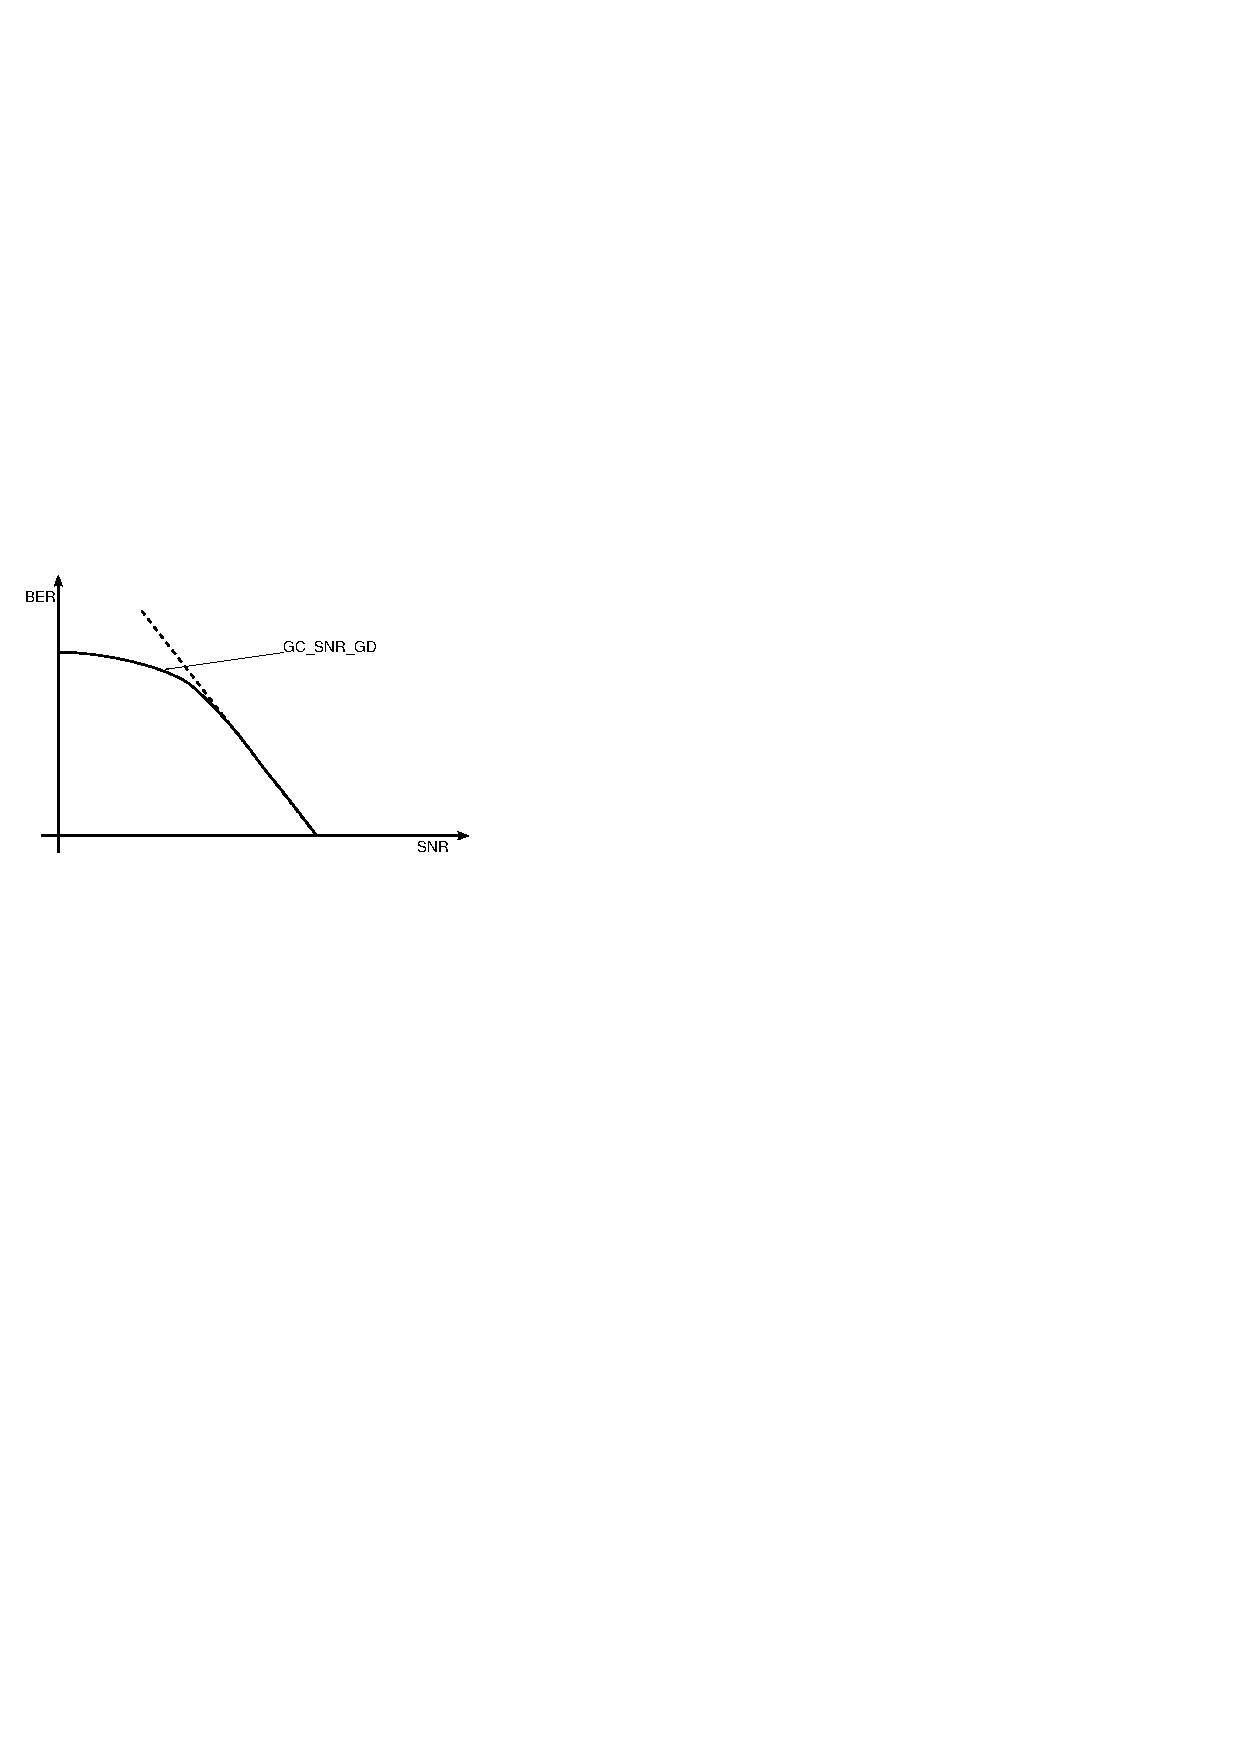
\includegraphics[width=7cm]{SIMO_BER_SNR_Kurve}
		\caption{Exemplary BER for SIMO}
		\label{fig:SIMO_BER_SNR_Kurve}
	
\end{minipage}
\hfill
\begin{minipage}[hbt]{5cm}
	\centering
		\begin{itemize}
			\item $G_c$ : Coding gain
			\item $G_d$ : Diversity gain
		\end{itemize}
\end{minipage}
\end{figure}

\subsubsection{Preliminaries}
Consider an equivalent system:
\begin{align*}
	y &= hx +n;\\
	\mathcal{E}\{|x^2|\} &= \mathcal{E}_s; & \mathcal{E}\{|n^2|\} &= \sigma_n^2; & \mathcal{E}\{|h|^2\} &= 1
\end{align*}
\begin{itemize}
	\item Instantaneous SNR: $\gamma_t = \frac{\mathcal{E}_s}{\sigma_n^2}\cdot |h|^2$
\item Average SNR: $\bar{\gamma}_t = \mathcal{E}\{\gamma_t\} = \frac{\mathcal{E}_s}{\sigma_n^2}$
\end{itemize}
\paragraph{Bit and Symbol Error Rate}
\begin{itemize}
	\item The Bit and Symbol Error Rate of many modulation schemes can be expressed for given $\gamma_t$ as:
\end{itemize}
\begin{align*}
	P_e(\gamma_t) = aQ\bigl( \sqrt{b\gamma_t}\bigr)
\end{align*}
where:
\begin{itemize}
	\item $Q(x) = \frac{1}{\sqrt{2\pi}}\cdot\int_{x}^{\infty} e^{-\frac{t^2}{2}}~dt$
	\item $P_e(\gamma_t)$ may be exact result or approximation
	\item BPSK: exact with $a = 1, b = 2$
	\item M-ary QAM: tight approximation with $a = 4\bigl (1-\frac{1}{\sqrt{M}}\bigr ), b =  \frac{3}{M - 1}$
\end{itemize}
\begin{math} \bigl ({\small Einschub: Gray-Code: {BER} = \frac{1}{\log_2M} \cdot {SER} }\bigr ) \end{math}
\begin{itemize}
	\item Alternative representation of Q\;-\;function:
			\begin{align*} 
			Q(x) = \frac{1}{\pi}\int_{0}^{\frac{\pi}{2}} e^{-\frac{x^2}{2\sin^2\theta}}~d\theta
			\end{align*}
			$\rightarrow$ Integral limits are fixed and do not depend on integration variables!
	\item Average error probability
		\begin{align*} 
		P_e = \mathcal{E}\bigl \{P_e(\gamma_t)\bigr \} = \int_{0}^{\infty}aQ\bigr (\sqrt{bx}\bigl )p_{\gamma_t}(x)~\mathrm{d}x
		\end{align*}
		\begin{itemize}
			\item Integral may be difficult to solve analytically
			\item Integral has infinite support $\rightarrow$ numerical evaluation difficult
		\end{itemize}
	\item Using alternative representation of Q-function we get:
		\begin{align*}
			P_e &= \int_{0}^{\infty}\frac{a}{\pi}\int_{0}^{\frac{\pi}{2}}e^{-\frac{bx}{2\sin^2\theta}}p_{\gamma_t}(x)~d\theta ~dx\\
			&= \frac{a}{\pi}\int_{0}^{\frac{\pi}{2}}\int_{0}^{\infty}p_{\gamma_t}(x)e^{-\frac{b}{2\sin^2\theta}x}~dx~d\theta &= \frac{a}{\pi}\int_{0}^{\frac{\pi}{2}}M_{\gamma_t}\bigl ( \frac{b}{2\sin^2\theta} \bigr )~d\theta
		\end{align*}
where:
		\begin{itemize}
				\item $M_{\gamma_t}(s) = \int_{0}^{\infty}p_{\gamma_t}(x)e^{-sx}~dx$ is the Laplace transform of $p_{\gamma_t}$	
				\item $M_{\gamma_t}(-s)$ is the so called Moment Generation Function (MGF) of $p_{\gamma_t}$
				\item Here, we will also refer to $M_{\gamma_t}(s)$ as MGF
				\item $M_{\gamma_t}(s)$ is sometimes easier to obtain than $p_{\gamma_t}$
				\item The above integral can be easily evaluated numerically because of the finite integral limits
			\end{itemize}
\end{itemize}
\paragraph{Outage probability}
\begin{itemize}
	\item The outage probability is the probability that the channel cannot support a certain rate, R, i.e. (where \begin{math} \gamma_T \end{math} is the threshold SNR):
		\begin{align*}
			C = \log_2(1+\gamma_t) < R \quad \leftrightarrow \quad \gamma_t < 2^R - 1 \hat{=} \gamma_T
		\end{align*}\\
		Thus, the outage probability is given by:
		\begin{align*}
			P_{out} &= P_0 \{\gamma_t <\gamma_T\}  \,= \int_{0}^{\gamma_T}p_{\gamma_t}(x)~dx
		\end{align*}
\item Using the inverse Laplace Transform\\
\begin{minipage}[hbt]{7cm}
	\centering
		\begin{align*}
			p_{\gamma  _t}(x) = \frac{1}{2\pi j}\int_{c-j\omega}^{c+j\omega}M_{\gamma _t}(s)e^{sx}~dx
		\end{align*}
	where \begin{math} c > 0\end{math} is a small constant that lies in the region of convergence of the integral, we obtain:
\end{minipage}
\hfill
\begin{minipage}[hbt]{5cm}
	\centering
	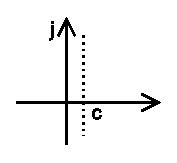
\includegraphics[width=2cm]{SIMO_Konstante_c}
\end{minipage}

\begin{itemize}
	\item 1.
			\begin{align*}
				P_{out} = \frac{1}{2\pi j}\int_{c-j\omega}^{c+j\omega}M_{\gamma _t}(s)\int_{0}^{\gamma _T}e^{sx}~dx~ds = \frac{1}{2\pi j}\int_{c-j\omega}^{c+j\omega}M_{\gamma _t}(s)e^{\gamma _Ts}~\frac{ds}{s}
			\end{align*}
			\begin{math}\bigl (\end{math}lower integral limit is 0 since \begin{math}p_{\gamma _t}(0) = 0 \bigr )\end{math}
	\item and 2.:
		\begin{align*}
			p_{\gamma _t} (x) &= \int_{0}^{x} p_{\gamma _t}(t) ~dt = 0\\		
		\text{for } x &= 0 \text{ note: } p_{\gamma _t}(x) \xleftrightarrow [transform]{Laplace} \frac{1}{s}M_{\gamma _t}(s)
		\end{align*}
	\end{itemize}
\end{itemize}
\paragraph{General combining scheme}
\begin{align*}
	y &= \Bigl (\sum_{n = 1}^{N_R}h_nw_n\Bigr )x + \sum_{n = 1}^{N_R}w_nn_n \\
	\gamma _t &= \frac{\mathcal{E}_s \Bigl | \sum_{n = 1}^{N_R}h_nw_n\Bigr |^2 }{\sigma _n^2 \sum_{n = 1}^{N_R}|w_n|^2}
\end{align*}
where \begin{math} w_n\end{math} depends on the particular combining scheme.
\subsubsection{MRC (Maximum Ratio Combining)}
\begin{itemize}
	\item what weight \begin{math}w_n\end{math} maximize \begin{math}\gamma _t\end{math}?
	\begin{itemize}
		\item Cauchy-Schwarz inequality
		\begin{align*}
			\Bigl | \sum_{n = 1}^{N_R}h_nw_n\Bigr |^2 \leq \sum_{n = 1}^{N_R}|h_n|^2 \cdot \sum_{n = 1}^{N_R}|w_n|^2
		\end{align*}
	where equality holds if and only if \begin{math}w_n = c\cdot h_n^*\end{math} for some non-zero constant \begin{math}c\end{math}.
		\item for \begin{math}w_n = h_n^*\end{math}, we obtain
		\begin{align*}
			\gamma _t = \frac{\mathcal{E}_s}{\sigma _n^2}\cdot \frac{\Bigl ( \sum_{n = 1}^{N_R}|h_n|^2\Bigr ) ^2}{\sum_{n = 1}^{N_R}|h_n|^2} = \frac{\mathcal{E}_s}{\sigma _n^2}\sum_{n = 1}^{N_R}|h_n|^2
		\end{align*}
		\item \begin{math}w_n = h_n^*\, \forall \, n\end{math} are the MRC combining weights.	
	\end{itemize}
	\item For performance analysis we assume \underline{independent identically distributed (IID)} Rayleigh fading
		\begin{align*}
			\rightarrow \mathcal{E}\{|h_n|^2\} &= 1; \quad \bar{\gamma} = \frac{\mathcal{E}_s}{\sigma	_n^2}; \quad \gamma _n = \frac{\mathcal{E}_s}{\sigma _n^2}|h_n|^2\\
			p_{\gamma}(x) &= \frac{1}{\bar{\gamma}}e^{-\frac{x}{\bar{\gamma}}}; \quad x\geq 0\\
			M_{\gamma}(s) &= \frac{1}{1+s\bar{\gamma}}
		\end{align*}		
	\item Error rate
			\begin{align*}
				\gamma _t = \sum_{n = 1}^{N_R}\gamma _n
			\end{align*}
			\begin{math}\rightarrow \end{math} sum of IID random variables (r.v.s.)
			\begin{align*}
				M_{\gamma _t}(s) = \Bigl (M_\gamma (s)\Bigr )^{N_R} = \frac{1}{(1 + s\bar{\gamma})^{N_R}} = \frac{1}{\bar{\gamma}^{N_R}}\cdot \frac{1}{(s + \frac{1}{\bar{\gamma}})^{N_R}}
			\end{align*}
			inverse Laplace-transform (from tables)
			\begin{align*}
				p_{\gamma _t}(x) = \frac{1}{\bar{\gamma}^{N_R}}\cdot \frac{x^{N_R-1}}{(N_R - 1)!}e^{-\frac{x}{\bar{\gamma}}};\quad x\geq 0
			\end{align*}
	\item Direct approach 
		\begin{align*}
			P_e &= \int_{0}^{\infty}a\cdot Q\bigl (\sqrt{ax} \bigr )p_{\gamma _t}(x)~dx = a\Bigl (\frac{1 - \mu}{2}\Bigr )^{N_R} \cdot \sum_{n = 0}^{N_R - 1}\begin{pmatrix} N_R - 1 + n \\ n\end{pmatrix}\Bigl (\frac{1 + \mu}{2}\Bigr )^n \\ \text{where}\; \mu &= \sqrt{\frac{b\bar{\gamma}}{2 + b\bar{\gamma}}}
		\end{align*}
		\item MGF approach
			\begin{align*}
				P_e &= \frac{a}{\pi}\int_{0}^{\frac{\pi}{2}}M_{\gamma _t}\Bigl ( \frac{b}{2\sin ^2\theta}\Bigr )~d\theta \\
				&= \frac{a}{\pi}\int_{0}^{\frac{\pi}{2}}\frac{1}{\bar{\gamma}^{N_R}\bigl (\frac{b}{2\sin ^2\theta} + \frac{1}{\bar{\gamma}}\bigr )^{N_R}}~d\theta \quad \text{(numerisch berechnen!)}
			\end{align*}
			\item with high SNR: \quad \begin{math}\bar{\gamma}\rightarrow \infty \Longleftrightarrow \frac{1}{\bar{\gamma}}\rightarrow 0 \end{math} and with MGF approach this leads to Average Error Probability $P_e$:
	\begin{align*}
		P_e &= \frac{a}{\pi}\cdot\frac{1}{\bar{\gamma}^{N_R}}\cdot \Bigl (\frac{2}{b}\Bigr )^{N_R}\int_{0}^{\frac{\pi}{2}}\sin ^{2N_R}\theta ~d\theta \\
		&= \frac{a}{2^{N_R+1}\cdot b^{N_R}}\begin{pmatrix}2N_R \\ N_R\end{pmatrix}\frac{1}{\bar{\gamma}^{N_R}}\quad \text{as } \bar{\gamma} \rightarrow \infty \\ 
		&\stackrel{!}{=} \Bigl (\frac{1}{G_c\bar{\gamma}}\Bigr )
	\end{align*}	
	where: 
	\begin{itemize}
		\item $ \int_{0}^{\frac{\pi}{2}}\sin ^{2N_R}\theta ~d\theta = \frac{\pi}{2^{N_R + 1}}\cdot \begin{pmatrix} 2N_R \\ N_R \end{pmatrix}$
		\item Diversity gain: $ G_d = N_R $ 
		\item Combining/Coding gain: $ G_c = 2b\biggl (\frac{a}{2}\begin{pmatrix}2N_R \\ N_R\end{pmatrix}\biggr )^{-\frac{1}{N_R}} $
	\end{itemize}		
	\begin{figure}[ht]
		\centering
		\psfrag{G_C}[hl][hl]{$G_c$}
		\psfrag{gamma_Mittelwert}[hl][hl]{$\bar{\gamma}$}
		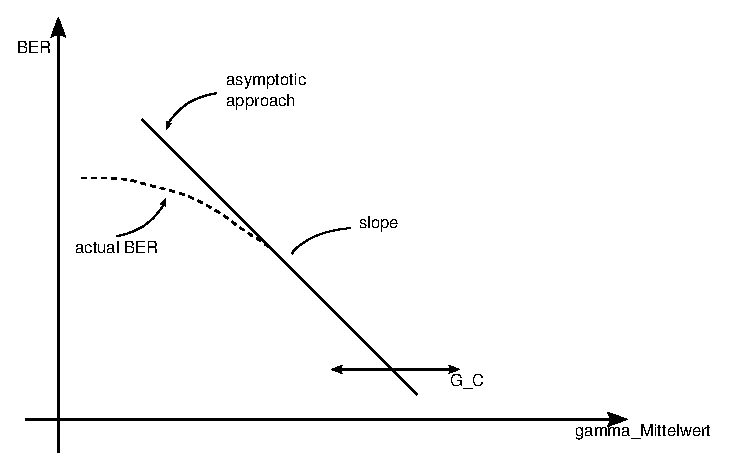
\includegraphics[width = 0.7\textwidth]{SIMO_BER_gamma_Kurve}
		\caption{BER for average SNR $\bar{\gamma_t}$}
		\label{fig:SIMO_BER_gamma_Kurve}
	\end{figure}
	\item MRC exploits the maximal possible diversity
	\item Diversity gain is not affected by correlation as the branches are not \underline{fully} correlated
	\item Diversity gain depends on fading distribution 
\end{itemize}
\paragraph{Outage probability}
\begin{align*}
	P_{out} &= \int_{0}^{\gamma _T}p_{\gamma _t}(x)~dx = \frac{1}{\bar{\gamma}^{N_R}}\int_{0}^{\gamma _T}\frac{x^{N_R-1}}{(N_R - 1)!}e^{-\frac{x}{\bar{\gamma}}}~dx \\ &= 1- e^{-\frac{\gamma _T}{\bar{\gamma}}}\cdot \sum_{n = 1}^{N_R}\frac{\bigl (\frac{\gamma _T}{\bar{\gamma}}\bigr )^n}{(n - 1)!}
\end{align*}
\begin{itemize}
	\item Approximation (Taylor series): $\bar{\gamma}\rightarrow \infty : -e^{-\frac{x}{\bar{\gamma}}} = 1 - \frac{x}{\bar{\gamma}} + O(\frac{1}{\bar{\gamma}})$\; where a function $f(x) \text{ is } O(x) \text{ if } \lim\limits_{x\to\infty}\frac{f(x)}{x} = 0$.
\begin{align*}
	\Rightarrow P_{out}=\frac{1}{\gamma^{N_R}}\int\limits_0^{\gamma_T}\frac{x^{N_R-1}}{(N_R-1)!}\left(1-\frac{x}{\bar{\gamma}}+O\left(\frac{1}{\bar{\gamma}}\right)\right)
\end{align*}
	\item Diversity and coding gain can also be defined for $P_{out}$
\end{itemize}

\subsubsection{EGC (Equal Gain Combining)}

\paragraph{Combining Weights}
\begin{itemize}
	\item For MRC, both, the amplitudes and phases of the channel gains $h_n=|h_n|e^{j\varphi_n}$ have to be known (or estimated in practice)
	\item In EGC it is assumed that only the phases are known and weights $w_n=e^{-j\varphi_n}$ are used.
\begin{align*}
	\Rightarrow \gamma_t &=\dfrac{\mathcal{E}_s}{\sigma_n^2}\dfrac{\left|\sum\limits_{n=1}^{N_R}|h_n|e^{j\varphi_n}e^{-j\varphi_n}\right|^2}{\sum\limits^{N_R}_{n=1}\left|e^{-j\varphi_n}\right|^2}
	=\frac{\mathcal{E}_s}{\sigma_n^2}\frac{1}{N_R}\left(\sum\limits^{N_R}_{n=1}|h_n|\right)^2\\
	&=\frac{1}{N_R}\left(\sum\limits_{n=1}^{N_R}\sqrt{\gamma_n}\right)^2;\text{  with  }\gamma_n=\frac{\mathcal{E}_s}{\sigma_n^2}|h_n|^2
\end{align*}
\end{itemize}
\paragraph{Performance Analysis}
\begin{itemize}
	\item IID case \\
	$\Rightarrow$ $\sqrt{\gamma_n}$ is Rayleigh distributed\\
	$\Rightarrow$ Exact analysis is much more difficult than for MRC $\Rightarrow$ see book by Simon\;\&\;Alouini p.341
	\item Approximate result
\begin{align*}
	P_e=\frac{a}{2}\left[1-\sqrt{\frac{2b\bar{\gamma}}{5+2b\bar{\gamma}}}\sum\limits_{n=0}^{N_R-1}\frac{\left(\! \begin{array}{c} 2n \\ n \end{array} \!\right) }{4^n(1+\frac{2}{5}b\bar{\gamma})^n}\right]
\end{align*}
	\item high SNR\\
	$\Rightarrow$ use high SNR analysis of Wang\;\&\;Giannakis, 2003\\
	$\Rightarrow$ at high SNR, only pdf of $\gamma_n$ around $0$ is relevant for performance
\begin{align*}
	\Rightarrow \overset{\text{Rayleigh}}{p_\gamma(x)} = \frac{1}{\bar{\gamma}}e^{-\frac{x}{\bar{\gamma}}}\overset{\text{Taylor Serie}}{=}\frac{1}{\bar{\gamma}}+O\left(\frac{1}{\bar{\gamma}}\right)\text{ as } x \to 0
\end{align*}
	\item need pdf $\gamma _t$: ($\gamma _n$ bekannt, $\rightarrow$ ges.: Wurzel, etc.)\\ (cumulative distribution function of $\sqrt{\gamma} $ (cdf))
	\begin{align*}
	% 1. Formel
		P_{\sqrt{\gamma}}(x) &= \text{Pr}\bigl\{\sqrt{\gamma}\leq x \bigr\} = \text{Pr}\bigl\{\gamma\leq x^2 \bigr\} = P_{\gamma}(x^2) = \text{cdf of}\;\gamma\\
	% 2. Formel
		\rightarrow p_{\sqrt{\gamma}}(x) &= \frac{d}{dx}P_{\sqrt{\gamma}}(x) = 2x\cdot p_{\gamma}(x^2) = \frac{2x}{\bar{\gamma}} + O\bigl(\frac{1}{\bar{\gamma}}\bigr)\\
	\end{align*}
	\item Laplace Transformation to MGF
	\begin{align*}
	% 3. Formel
		\rightarrow M_{\sqrt{\gamma}}(s) &= \mathcal{L}\bigl\{p_{\sqrt{\gamma}}(x)\bigr\} = \frac{2}{\bar{\gamma}}\cdot \frac{1}{s^2} + O\bigl(\frac{1}{\bar{\gamma}}\bigr)\\
	% 4. Formel
		\sqrt{\gamma _t} &= \sum_{n = 1}^{N_R}\frac{\sqrt{\gamma _n}}{N_R}\\
	% 5. Formel
		 M_{\sqrt{\gamma _t}}(s) &= \mathcal{E}\Bigl\{\mathrm{exp}({-s\sqrt{\gamma _t}})\Bigr\} = \mathcal{E}\Bigl\{\mathrm{exp}({-\frac{s}{\sqrt{N_R}}\cdot \sum_{n = 1}^{N_R}\sqrt{\gamma _n}})\Bigr\} = \Bigl(\mathcal{E}\Bigl\{\mathrm{exp}(-\frac{s}{\sqrt{N_R}}\cdot \sqrt{\gamma _n}\Bigr\}\Bigr)^{N_R}\\
	% 6. Formel
		 &= \Bigl( M_{\sqrt{\gamma}}\bigl(\frac{s}{\sqrt{N_R}}\bigr) \Bigr)^{N_R} = \Bigl(\frac{2}{\bar{\gamma}}\cdot \frac{N_R}{s^2}\Bigr)^{N_R} + O\Bigl(\frac{1}{\bar{\gamma}^{N_R}}\Bigr)\\
	\end{align*}
	\item inverse Laplace Transform
	\begin{align*}
	% 7. Formel
		p_{\sqrt{\gamma _t}}(x) &= \mathcal{L} ^{-1}\Bigl\{M_{\sqrt{\gamma _t}}(s)\Bigr\} = \Bigl(\frac{2N_R}{\bar{\gamma}}\Bigr)^{N_R}\cdot \frac{x^{2N_R-1}}{(2N_R-1)!} + O\Bigl(	\frac{1}{\bar{\gamma}^{N_R}}\Bigr)\\
	% 8. Formel
		P_{\gamma _t}(x) &= \text{Pr}\bigl\{\gamma _t\leq x	\bigr\} =  \text{Pr}\bigl\{\sqrt{\gamma _t}\leq \sqrt{x}\bigr\} = P_{\sqrt\gamma _t}(\sqrt{x}) \rightarrow \text{cdf of } \sqrt{\gamma _t}\\
	% 9. Formel
		p_{\gamma _t}(x) &= \frac{d}{dx}P_{\gamma _t}(x) = \frac{1}{2\sqrt{x}}\cdot p_{\gamma _t}(\sqrt{x}) = \frac{1}{2}\Bigl(\frac{2N_R}{\bar{\gamma}} \Bigr)^{N_R}\cdot \frac{x^{N_R-1}}{(2N_R-1)!} + O\bigl(\bar{\gamma}^{-N_R}\bigr)\\
	% 10. Formel
		\rightarrow M_{\gamma _t}(s) &= \mathcal{L}\bigl\{p_{\gamma _t}(x)\bigr\} = \frac{1}{2}\Bigl( \frac{2N_R}{\bar{\gamma}}\Bigr)^{N_R}\cdot \frac{(N_R - 1)!}{(2N_R -1)!~b^{N_R}} + O\bigl(\bar{\gamma}^{-N_R}\bigr)\\
	% 11. Formel
	\end{align*}
	\item Error Probability:
\begin{align*}
        P_e&=\frac{a}{\pi}\int\limits_0^{\frac{\pi}{2}}M_{\gamma_t}\left(\frac{b}{2\sin^2(\theta)}\right)\mathrm{d}\theta\\
        &=\frac{a}{\pi}\frac{1}{2}\left(\frac{2N_R}{\bar{\gamma}}\right)^{N_R}\frac{(N_R-1)!}{(2N_R-1)!}
        \frac{2^{N_R}}{b^{N_R}}
        \underbrace{\int\limits_0^{\frac{\pi}{2}}\sin^{2N_R}(\theta)\mathrm{d}\theta}_
        {\frac{\pi}{2^{2N_R+1}}\binom{2N_R}{N_R}=\frac{\pi(2N_R)!}{2^{2N_R+1}(N_R!)^2}}
        +O\left(\frac{1}{\bar{\gamma}^{N_R}}\right)\\
        &= \frac{aN_R^{N_R}}{2b^{N_R}N_R!}\frac{1}{\bar{\gamma}^{N_R}}+O\left(\frac{1}{\bar{\gamma}^{N_R}}\right)
        \overset{!}{=}\left(\frac{1}{G_c\cdot\bar{\gamma}}\right)^{G_d}
\end{align*}

\begin{itemize}
		\item[] $\Longrightarrow \text{Diversity gain: } G_d = N_R$
		\item[] $\Longrightarrow \text{Combining gain: } G_c = \frac{b}{N_R}\Bigl( \frac{2N_R!}{a}\Bigr)^{\frac{1}{N_R}}$
		\item[] vergleiche auch Blatt mit Kurven \Rmnum{3} und \Rmnum{4}
	\end{itemize}
\end{itemize}
A similar asymptotic analysis can be conducted for the outage probability.
\subsubsection{SC (Selection Combining)}
\paragraph{Combining weights}
	\begin{itemize}
		\item only the strongest branch is chosen
		\item strongest branch: $\hat{n} = \underset{n}{\text{argmax}} \gamma _n \longrightarrow \gamma _t = \gamma _{\hat{n}}$
		\item only on RF receiver chain required $\rightarrow$\; saves hardware complexity 
	\end{itemize}
\paragraph{Performance analysis}
	\begin{itemize}
		\item cdf of: $\gamma _t$
			\begin{align*}
				P_{\gamma _t}(x) &= \text{Pr}\bigl\{\gamma _{\hat{n}} \leq x\bigr\} = \text{Pr}\bigl\{\gamma _1 \leq x \cap \gamma _2 \leq x \cap \dots \gamma _{N_R} \leq x\bigr\}\\
				&\overset{(IID)}{=} \Bigl(\text{Pr}\bigl\{\gamma _n \leq x\bigr\}\Bigr)^{N_R} = \Bigl( P_{\gamma}(x)\Bigr)^{N_R}
			\end{align*}
		\item pdf:
			\begin{align*}
				p_{\gamma _t}(x) &= \frac{d}{dx}P_{\gamma _t}(x) = N_R\bigl(P_{\gamma}(x)\bigr)^{N_R-1}\cdot p_{\gamma}(x)\\
				\text{where: }\qquad p_{\gamma} (x) &= \frac{1}{\bar{\gamma}}e^{-\frac{x}{\bar{\gamma}}};\quad x\geq 0\\
				P_{\gamma}(x) &= \int_{0}^{x}p_{\gamma}(x)~dx = 1 - e^{-\frac{x}{\bar{\gamma}}};\quad x\geq 0\\
				\rightarrow p_{\gamma _t}(x) &= \frac{N_R}{\bar{\gamma}}\bigl( 1 - e^{-\frac{x}{\bar{\gamma}}}\bigr)^{N_R-1}e^{-\frac{x}{\bar{\gamma}}};\quad x\geq 0
			\end{align*}
	\end{itemize}
\paragraph{Error probability}
	\begin{itemize}
		\item direct approach $\rightarrow$ closed-form solution possible
		\item MGF approach (with Binomial expansion):
			\begin{align*}
				p_{\gamma _t}(x) &= \frac{N_R}{\bar{\gamma}}e^{-\frac{x}{\bar{\gamma}}}\sum_{n = 0}^{N_R - 1}\begin{pmatrix} N_R - 1 \\ n\end{pmatrix} 1^{N_R - 1 - n}\Bigl( -e^{-\frac{x}{\bar{\gamma}}}\Bigr)^n \\ 
				&= \frac{N_R}{\bar{\gamma}}\sum_{n = 0}^{N_R - 1}\begin{pmatrix}N_R - 1 \\ n\end{pmatrix}\cdot (-1)^{n}e^{-\frac{x(n + 1)}{\bar{\gamma}}};\quad	x \geq 0 \\ \\
				M_{\gamma_t}(s) &= \frac{N_R}{\bar{\gamma}}\sum_{n = 0}^{N_R - 1}\begin{pmatrix}N_R - 1\\n\end{pmatrix}(-1)^{n}\frac{1}{s + \frac{n+1}{\bar{\gamma}}}\\ \\
				P_e &= \frac{a}{\pi}\int_{0}^{\frac{\pi}{2}}M_{\gamma _t}\Bigl(\frac{b}{2\sin^2\theta}\Bigr)~d\theta = \frac{aN_R}{\pi\bar{\gamma}}\sum_{n = 0}^{N_R - 1}\begin{pmatrix}N_R - 1\\ n\end{pmatrix} (-1)^{n}\int_{0}^{\frac{\pi}{2}}\frac{\mathrm{d}\theta}{\frac{b}{2\sin^2\theta} + \frac{n + 1}{\bar{\gamma}}}\\ &\rightarrow\text{can be evaluated numerically}				
			\end{align*}
		\item high SNR approach $\Rightarrow \; \bar{\gamma}\rightarrow\infty$
			\begin{align*}
			p_{\gamma_t}
			&=\frac{N_R}{\bar{\gamma}}
			\left[1-\mathrm{exp}\left(-\frac{x}{\bar{\gamma}}\right)\right]^{N_R-1}\mathrm{exp}\left(-\frac{x}{\bar{\gamma}}\right)\\
			&\overset{\bar{\gamma} \rightarrow \infty}{=} \frac{N_R}{\bar{\gamma}}
			\left[1-\left(1-\frac{x}{\bar{\gamma}}+O\left(\bar{\gamma}^{-1}\right)\right)\right]^{N_R-1}
			\left(1-\frac{x}{\bar{\gamma}}+O\left(\bar{\gamma}^{-1}\right)\right)\\
			&=\frac{N_R}{\bar{\gamma}^{N_R}}x^{N_R-1}+o\left(\bar{\gamma}^{-N_R}\right)\\ \\
			M_{\gamma_t}(s)
			&=\frac{N_R}{\bar{\gamma}^{N_R}}\frac{(N_R-1)!}{s^{N_R}}+O\left(\bar{\gamma}^{-N_R}\right)\\
			\Bigl[\rightarrow P_e
			&=\frac{a}{\pi}\int\limits^{\frac{\pi}{2}}_0 M_{\gamma_t}\left(\frac{b}{2\sin^2(\theta)}\right)\mathrm{d}\theta\Bigr]\\
			&=\frac{a(2N_R)!}{b^{N_R}2^{N_R+1}N_R!}\frac{1}{\bar{\gamma}^{N_R}}+O(\bar{\gamma}^{-N_R})
			\end{align*}
		\begin{itemize}
			\item[] $\Longrightarrow \text{Diversity gain: } G_d = N_R$
			\item[] $\Longrightarrow \text{Combining gain: } G_c = 2b\left(\frac{2N_R!}{a(2N_R)!}\right)^{\frac{1}{N_R}}$
			%\item[] vergleiche auch Blatt mit Kurven \rom{III} und \rom{IV}
		\end{itemize}
	\end{itemize}

\paragraph{Outage Probability}
		\begin{align*}
			P_{out}&=\mathrm{Pr}\{\gamma_{\hat{n}} \leq \gamma_T \}=P_{\gamma_{\hat{n}}}(\gamma_T)=\left[1-\mathrm{exp}\left(-\frac{\gamma_T}{\bar{\gamma}}\right)\right]^{N_R}\\
			\text{high SNR: } P_{out}&=\left(\frac{\gamma_T}{\bar{\gamma}}\right)^{N_R}+O\left(\bar{\gamma}^{-N_R}\right)
		\end{align*}

\subsubsection{Comparison}
	\begin{itemize}
		\item Diversity Gain:\\
			MRC, EGC and SC all achieve the maximum possible diversity gain of $G_d=N_R$
		\item Combining Gain:\\
			The combining gains of MRC, EGC and SC are different
			\begin{itemize}
			\item MRC/EGC:
			\begin{align*}
			\frac{G_C^{EGC}}{G_C^{MRC}}=\frac{\frac{1}{2b}\left(\frac{a}{2}\binom{2N_R}{N_R}\right)^{\frac{1}{N_R}}}{\frac{N_R}{b}\left(\frac{a}{2}\frac{1}{N_R!}\right)^{\frac{1}{N_R}}}
			=\frac{[(2N_R)!]^{\frac{1}{N_R}}}{2N_R(N_R)^{\frac{1}{N_R}}}\leq 1\\
			\end{align*}
			(independent of a or b which are modulation parameters, only depends on number of antennas)
			\begin{align*}
				N_R \gg 1: \qquad N_R!\approx \sqrt{2\pi}e^{-N_R}N_R^{N_R+\frac{1}{2}}\qquad(Stirling)
			\end{align*}
			\begin{align*}
				\left.\frac{G_c^{EGC}}{G_c^{MRC}}\right|_{N_R\gg1}
				=\frac{\left(\sqrt{2\pi}e^{-2N_R}(2N_R)^{2N_R+\frac{1}{2}}\right)^{\frac{1}{N_R}}}{2N_R\left(\sqrt{2\pi}e^{-N_R}N_R^{N_R+\frac{1}{2}}\right)^{\frac{1}{N_R}}}
				=\frac{2\cdot2^{\frac{1}{2N_R}}}{2}\overset{N_R\rightarrow\infty}{\rightarrow}\frac{2}{e}\equiv -1.3\mathrm{dB}
			\end{align*}
			\item MRC/SC:
			\begin{align*}
				\frac{G_c^{SC}}{G_c^{MRC}}
				&=\frac{2b\left(\frac{a}{2}\binom{2N_R}{N_R}\right)^{\frac{1}{N_R}}}{2b\left(\frac{a}{2}\frac{(2N_R)!}{N_R!}\right)^{\frac{1}{N_R}}}
				=\frac{1}{(N_R!)^{\frac{1}{N_R}}} \leq 1\\
				\left.\frac{G_c^{SC}}{G_c^{MRC}}\right|_{N_R\gg1}&=\frac{1}{\sqrt{2\pi}^{\frac{1}{N_R}}e^{-1}N_R^{1+\frac{1}{2N_R}}}\overset{\rightarrow}{N_R\rightarrow\infty}\frac{e}{N_R}
			\end{align*}
			$\rightarrow$ loss increases with $N_R$
			\end{itemize}
		\item Ergebnis:
		\begin{itemize}
			\item unterschiedliche Kurven in Diagramm \glqq Combiner Performance Comparison, BPSK\grqq\ ergeben sich durch $G_c$
			\item alle Kurven haben die gleiche Steigung $\Rightarrow G_d $ ist \"uberall gleich
			\item nur Abst\"ande sind unterschiedlich $\Rightarrow G_c $ wird in MRC besser \glqq genutzt\grqq\ als in EGC und SC
		\end{itemize}
	\end{itemize}
	\newpage
\subsection{MISO Systems}
\paragraph{Remarks}
	\begin{itemize}
		\item Similar to SIMO systems, in MISO systems only coding and diversity gains can be obtained.
		\item To realize these gains, a careful transmitter design is necessary
		\item System design depends on whether or not channel state information (\textbf{CSI}) is available at transmitter
	\end{itemize}
\subsubsection{Naive Approach}
\begin{itemize}	
	\item Assume we simply send the same signal over all $N_T$ transmit antennas
\end{itemize}
\begin{figure}[ht]
	\centering
	\input{MISO_NAIVE.pstex_t}
	\caption{Block Diagramm of naive MISO}
	\label{fig:MISO_NAIVE.pstex_t}
\end{figure}

\begin{itemize}
	\item Transmit power: $\mathcal{E}\left\{\left|\frac{1}{\sqrt{N_T}}x\right|^2+,\dots,\left|\frac{1}{\sqrt{N_T}}x\right|^2\right\}=\mathcal{E}\left\{N_T\frac{1}{N_T}|x|^2\right\}=\mathcal{E}_s$
	\item Received signal: $y=\frac{1}{\sqrt{N_T}}\sum\limits_{n=1}^{N_T}h_n\cdot x+n$
	\item Rayleigh fading: $h_n$ are zero mean complex gaussian random variables\\
	$\rightarrow$ $h$ is also zero mean complex gaussian
	\item i.i.d.:
	\begin{itemize}
		\item $\mathcal{E}\{|h_n|^2\}=1\;\forall n$
		\item $\mathcal{E}\{|h|^2\}=\frac{1}{N_T}\mathcal{E}\left\{\left|\sum\limits_{n=1}^{N_T}h_n\right|^2\right\}=\frac{1}{N_T}\mathcal{E}\left\{\sum\limits^{N_T}_{n=1}|h_n|^2\right\}=1$
		\item statistical properties of h are independent of $N_T$
		\item the multiple transmit antennas have no benefit at all
		\item \underline{more sophisticated transmitter designs necessary}
	\end{itemize}
\end{itemize}
\subsubsection{Full CSI Available at the Transmitter}
\begin{itemize}
	\item $h_n, n \in \{1,\dots,N_T\}$ is known at the transmitter
	\item Perform ``precoding'' (beamforming) with coefficients $w_n$
\end{itemize}
\begin{figure}[ht]
	\input{MISO_CSI.pstex_t}	
	\caption{Block Diagramm of MISO with CSI}
	\label{fig:MISO_CSI.pstex_t}
\end{figure}

\begin{itemize}
	\item Transmit Power: Two constraints maybe considered
	\begin{itemize}
		\item Average transmit power constraint
		\begin{align*}
		P_{av}=\mathcal{E}\left\{\sum\limits^{N_T}_{n=1}|w_n^*x|^2\right\}=\sum\limits_{n=1}^{N_T}|w_n|^2\underbrace{\mathcal{E}\{|x|^2\}}_{\mathcal{E}_s}=\mathcal{E}_s \Rightarrow \sum\limits^{N_T}_{n=1}|w_n|^2=1
		\end{align*}
		\item Power constraint for each transmit antenna
		\begin{align*}
		\rightarrow |w_n|=\frac{1}{\sqrt{N_T}} \qquad \rightarrow P_{av}=\mathcal{E}_s
		\end{align*}
	\end{itemize}
	\item Recveived signal: $y=\underbrace{\sum\limits^{N_T}_{n=1}w^*_nh_n}_{h}x+n$ (equivalent SISO channel)
\end{itemize}
\paragraph{Maximum Ratio Transmission (MRT)}
\begin{itemize}
	\item we have only the average power constraint: $ \sum_{n = 1}^{N_T} |w_n|^2 = 1 $
	\item SNR:  $\gamma	 _t = \frac{\mathcal{E}_s|h|^2}{\sigma _n^2} = \frac{\mathcal{E}_s\left|\sum_{n = 1}^{N_T}w_n^*\cdot h_n \right|^2}{\sigma _n^2} $ 
	\item Maximize SNR under constraint $ \sum_{n = 1}^{N_T}|w_n|^2 = 1 $
	\item constraint optimization problem $\rightarrow $ Lagrange method
		\begin{align*}
			L = \frac{\mathcal{E}_s}{\sigma _n^2}\left| \sum_{n = 1}^{N_T}w_n^*\cdot h_n \right |^2 + \lambda\left ( \sum_{n = 1}^{N_T}|w_n|^2 - 1\right ); \quad \text{where: } \lambda = \text{Lagrange Multiplier}
		\end{align*}
		$\Rightarrow$  Wirtinger Kalk\"ul: treat  $z$  and  $z^*$  as independent variables for differentiation:
		\begin{align*}
			\frac{\partial z^*}{\partial z} &= 0;\quad  \frac{\partial |z|^2}{\partial z} = \frac{\partial z\cdot z^*}{\partial z} = z^*\\
			\frac{\partial x^2}{\partial x} &= 2x; \quad \frac{\partial (z^*)^2}{\partial z^*} = 2\cdot z^*;  \frac{\partial |z|^2}{\partial z} = z^*
		\end{align*}
		\begin{align*}
			\frac{\partial L}{\partial w_m^*} = \frac{\mathcal{E}_s}{\sigma _n^2}\Bigl ( \sum_{n = 1}^{N_T}w_n^*\cdot h_n\Bigr )^*h_m + \lambda w_m
		\end{align*}
		\begin{itemize}
			\item[$\rightarrow$] $   w_m =\underset{\text{const., independent of } m:=c}{\frac{\mathcal{E}_s}{\sigma _n^2 \cdot \lambda}\Bigl ( \sum\limits_{n = 1}^{N_T}w_n^*h_n \Bigr )^*}h_m $
			\item[$\rightarrow$] $  w_m = c\cdot h_m$
			\item[$\rightarrow$] $ \sum_{n = 1}^{N_T} |w_n|^2 = 1 \rightarrow c^2 = \frac{1}{\sum\limits_{n = 1}^{N_T}|h_n|^2}  $
			\item[$\rightarrow$] $  w_n = \frac{h_n}{\sqrt{\sum_{n = 1}^{N_T}|h_n|^2}} \equiv $ MRT gains 
		\end{itemize}
		\item[$\rightarrow$] SNR $ = \frac{\mathcal{E}_s}{\sigma _n^2}\Bigl | \sum_{n = 1}^{N_T}\frac{|h_n|^2}{\sqrt{\sum_{m = 1}^{N_T}|h_m|^2}}\Bigr |^2 = \frac{\mathcal{E}_s}{\sigma _n^2}\sum_{n = 1}^{N_T}|h_n|^2 $
		\item[$\Rightarrow$] same SNR as for maximum ration combining (MRC)
		\item[$\Rightarrow$] MRT with $N_T$ transmit antennas achieves the same performance as MRC with $N_T$ receive antennas
		\item[$\Rightarrow$] MRT/MRC can be extended to $ N_T\times N_R $ MIMO systems
		\begin{itemize}
			\item[$\rightarrow$] has the same performance as MRC with $N_T\cdot N_R$ receive antennas and one transmit antenna
		\end{itemize}
	\end{itemize}
\paragraph{Equal Gain Transmission (EGT)}
\begin{itemize}
	\item we employ gains: $w_n = \frac{1}{\sqrt{N_T}}\cdot \frac{h_n}{|h_n|} \rightarrow |w_n| = \frac{1}{\sqrt{N_T}} $
	\item SNR:
	\begin{align*}
		\gamma _t 
		&= \frac{\mathcal{E}_s}{\sigma _n^2}\left|\sum_{n = 1}^{N_T} w_n^*h_n \right |^2\\
		&= \frac{\mathcal{E}_s}{\sigma _n^2}\left|\sum_{n = 1}^{N_T}\frac{1}{\sqrt{N_T}}\cdot \frac{|h_n|^2}{|h_n|} \right|^2 = \frac{1}{N_T}\cdot \frac{\mathcal{E}_s}{\sigma _n^2} \left|\sum_{n = 1}^{N_T}|h_n| \right|^2\\
		\gamma _n 
		&= \frac{\mathcal{E}_s}{\sigma _n^2}|h_n|^2\\
		&\text{same SNR as for EGC} \rightarrow \gamma _t = \frac{1}{N_T} \left| \sum_{n = 1}{N_T}\sqrt{\gamma _n} \right|^2
	\end{align*}
	\item[$\rightarrow$] EGC with $ N_T$ transmit antennas achieves the same performance as EGC with $ N_T$ receive antennas
\end{itemize}
\paragraph{Transmit Antennas Selection}
\begin{itemize}
	\item select antenna with maximum channel gain for transmission:
		\begin{align*} 
			w_n = 
			\begin{cases}
\frac{h_n}{|h_n|},  & \text{if } n = \hat{n}\\
0, & \text{otherwise}
\end{cases} \text{where } \hat{n} = \underset{n}{\mathrm{argmax}}|h_n|
		\end{align*}
	\item antenna selection with $ N_T$ transmit antennas achieves the same performance as \textit{Selection Combining} with $ N_T$ receive antennas
\end{itemize}
\subsubsection{No CSI at Transmitter - Space\,-\,Time\,-\,Coding}
\begin{itemize}
	\item $h_n, n\in\{1,\dots ,N_T\}$, is only known at the receiver
	\item ``Space-time-coding'' has to be employed to realize diversity gain
	\item $T\times N_T$ matrics $\mathbf{X}$ are transmitted in $T$ symbol intervals over $N_T$ antennas
	\item $\mathbf{X}$ is drawn from a matrix alphabet $\mathcal{X}$
	\item Example:
	\begin{align*}
		\mathbf{X}=\begin{pmatrix} x_{1,1} & x_{1,2} & \cdots & x_{1,N_T} \\
					   x_{2,1} & x_{2,2} & \cdots & x_{2,N_T} \\
					   \vdots  & \vdots  & \ddots & \vdots    \\
				 	   x_{T,1} & x_{T,2} & \cdots & x_{T,N_T}
			\end{pmatrix}
	\end{align*}
	\item We distinguish:
		\begin{itemize}
			\item Space-time-block-codes (STBCs)\\
			$\rightarrow$ $\mathbf{X}$ is obtained by mapping $K$ scalar symbols $s_k,\; k=1, \dots , K$ from a scalar alphabet $\mathcal{A}$ to matrix $\mathbf{X}$
			\item Space-time-trellis-codes (STTCs)\\
			$\rightarrow$ $\mathbf{X}$ is obtained from scalar symbols $s_k$ through a trellis encoding process.\\
			{\small[see: Tarokh, Seshadri, Calderbank: Space-time-codes for high datarate wireless communication: Performance criterions and coder construction; IEEE Trans. Inf. Theory 1998]}
			\item here: We concentrate on space-time-block-codes (STBCs), but many results can be easily extended to space-time-trellis-codes
		\end{itemize}
	\item STBCs:
		\begin{itemize}
			\item  $K$ $M$-ary scalar symbols (e.g. $M$-PSK symbols) are mapped to STBC matrices $\mathbf{X}$\\ 
			$\mathbf{S}=[s_1,\dots ,s_K] \rightarrow \mathbf{X}$\\
			$s_k\in \mathcal{A} \rightarrow x\in\mathcal{X}$ with $|\mathcal{X}|=M^K$
			\item Example: ``Alamouti''-Code\\
			\begin{align*}
				\mathbf{X}=\frac{1}{\sqrt{2}}
				\begin{pmatrix}
					s_1 & s_2 \\
					-s_2^* & s_1^*
				\end{pmatrix}
			\end{align*}
			{\small[Alamouti: A simple transmit diversity technique for wireless communication, IEEE JSAC 1998]}
		\end{itemize}
\end{itemize}
\paragraph{Optimal Detection}
\begin{itemize}
	\item Signal model:
	\begin{align*}
	\begin{pmatrix} y_1 \\ \vdots \\ y_T \end{pmatrix}&=\mathbf{X}\begin{pmatrix} h_1 \\ \vdots \\ h_{N_T} \end{pmatrix} + \begin{pmatrix} n_1 \\ \vdots \\ n_T \end{pmatrix}\\
	\mathbf{y}&=\mathbf{X}\cdot\mathbf{h}+\mathbf{n}
	\end{align*}
	\item Optimal detection - ML-detection
	\begin{itemize}
		\item $\mathbf{h}$ is known at receiver
		\item $\mathbf{n}$ is AWGN with $\mathcal{E}\{\mathbf{n}\cdot\mathbf{n^H}\}=\sigma_{\mathbf{n}}^2\cdots \mathbf{I}_{T\times T}$
		\begin{align*}
		p(\mathbf{y}|\mathbf{X})
		&=\frac{1}{\pi^T|\sigma_n^2\mathbf{I}_{T\times T}|}\mathrm{exp}\left(-(\mathbf{y - Xh})^H(\sigma_n^2\mathbf{I}_{T\times T})^{-1}(\mathbf{y-Xh})\right)\\
		&=\frac{1}{\pi^T\sigma_n^{2T}}\mathrm{exp}\left(-\frac{1}{\sigma_n^2}(\mathbf{y-Xh})^H(\mathbf{y-Xh})\right)=\frac{1}{\pi^T\sigma_n^{2T}}\mathrm{exp}\left(||\mathbf{y-Xh}||^2\right)
		\end{align*}
		$\rightarrow$ the optimal estimate $\hat{\mathbf{X}}$ or equivalently the optimal estimate $\hat{\mathbf{s}}$ can be obtained as
		\begin{align*}
			\hat{\mathbf{s}}=\underset{\mathbf{s}\in\mathcal{A}^K}{\mathrm{argmax}}\;p(\mathbf{y|X})=\underset{\mathbf{s}\in\mathcal{A}^K}{\mathrm{argmin}}||\mathbf{y-Xh}||^2
		\end{align*}
		\item Disadvantage: In general, metric $||\mathbf{y-Xh}||^2$ has to be calculated $M^K$ times\\
		$\rightarrow$ complexity increases exponentially with $K$
	\end{itemize}
\end{itemize}
\paragraph{Types of STBCs}
\begin{itemize}
	\item Orthogonal STBCs (OSTBCs)
	\begin{itemize}
		\item OSTBCs are a special class of STBCs which allow independent detection of each $s_k \rightarrow$ only $K\cdot M$ metrics have to be evaluated
		\item Rate STBCs: $R_{STBC} = \frac{K}{T}$
		\item Examples:
		\begin{itemize}
			\item Alamouti Code  $(K = 2, T = 2) \rightarrow R_{STBC} = 1$
			\begin{align*}
				\textbf{X} &= \frac{1}{\sqrt{2}}\underset{\longleftrightarrow N_T}{\begin{pmatrix} s_1 & s_2 \\ -s_2^* & s_1^*	\end{pmatrix}}\updownarrow T\\
				\rightarrow &\text{ only ``full rate ´´ OSTBC for complex } s_k
			\end{align*}
			\item $N_T = 3, K = 3, T = 4$
			\begin{align*}
				\textbf{X} = \frac{1}{\sqrt{3}}\begin{pmatrix*}[r]	s_1 & s_2 & s_3 \\ -s_2^*  & s_1^* & 0 \\ s_3^* & 0 & -s_3^*\\0 & -s_3^* & s_2^*\end{pmatrix*} \rightarrow R_{STBC} = \frac{K}{T} = \frac{3}{4}
			\end{align*}
		\end{itemize}
		\item Orthogonality: $\textbf{X}^H\textbf{X} = {const}\cdot \textbf{I}_{N_T\times N_T}$
		\item Independent detection of $s_1$ \& $s_2$ for Alamouti Code
		\begin{align*}
				\begin{pmatrix*}[r]y_1 \\y_2 
			\end{pmatrix*} &= \frac{1}{\sqrt{2}}
			\begin{pmatrix*}[r]	s_1 & s_2 \\-s_2^* & s_1^*
			\end{pmatrix*}
			\begin{pmatrix*}[r]h_1\\h_2
			\end{pmatrix*} + 
			\begin{pmatrix*}[r]n_1\\n_2
			\end{pmatrix*}\\
			\rightarrow 
			\underbrace{
			\begin{pmatrix*}[r]y_1\\y_2
			\end{pmatrix*}}_{\tilde y} &= \frac{1}{\sqrt{2}}
			\underbrace{
			\begin{pmatrix*}[r]h_1 & h_2\\h_2^* & -h_1^*
			\end{pmatrix*}}_{\tilde F}
			\underbrace{
			\begin{pmatrix*}[r]s_1\\s_2
			\end{pmatrix*}}_{s} + 
			\underbrace{
			\begin{pmatrix*}[r]n_1\\n_2^*
			\end{pmatrix*}}_{\tilde n}
		\end{align*}
		$\Bigl ( $ Anmerkung: \underline{nur } $\begin{pmatrix}s_1 \\s_2 \end{pmatrix} $ gew\"unscht, nicht: $s_1^*, s_2^* \Bigr ) $
		\begin{align*}
			\textbf{F}^H\textbf{F} = \frac{1}{2}\begin{pmatrix}h_1^* & h_2\\h_2^* & -h_1\end{pmatrix}\begin{pmatrix}h_1 & h_2\\h_2^* & -h_1^* \end{pmatrix} = \frac{1}{2}\begin{pmatrix} |h_1|^2 + |h_2|^2 & 0\\0 & |h_1|^2 + |h_2|^2\end{pmatrix}		 								
		\end{align*}
		\begin{itemize}
			\item[$\rightarrow$] $\frac{\sqrt{2}}{\sqrt{|h_1|^2 + |h_2|^2}}\cdot \textbf{F} $ is unitary matrix 
			\item[$\rightarrow$] $\frac{2}{|h_1|^2 + |h_2|^2}\cdot \textbf{F}^H\cdot \tilde{\textbf{y}} = \textbf{s} + \frac{2}{|h_1|^2 + |h_2|^2}\cdot \textbf{F}^H\cdot\tilde{\textbf{n}}$ \\  $\bigl ( \frac{2}{|h_1|^2 + |h_2|^2}\cdot \textbf{F}^H\cdot\tilde{\textbf{n}}$ is AWGN vector with covariance matrix $\frac{2\sigma_n^2}{|h_1|^2 + |h_2|^2}\cdot \textbf{I}_{T\times T} \bigr)$
			\item[$\rightarrow$] ML decision: $\hat{\textbf{s}} = \underset{\textbf{s}}{\text{argmin}}\bigl | \bigl | \frac{2}{|h_1|^2 + |h_2|^2}\cdot \textbf{F}^H\cdot \tilde{\textbf{y}} - \textbf{s}\bigr |\bigr |^2 $
			\item[$\rightarrow$] independent ML decoding 
				\begin{align*}
					\hat{s}_1 &= \underset{s_1}{\text{argmin}} \Bigl |s_1 - \frac{h_1^*y_1 + h_2y_2^*}{\frac{1}{\sqrt{2}}(|h_1|^2 + |h_2|^2)}\Bigr |\\ \hat{s}_2 & = \underset{s_2}{\text{argmin}}\Bigl |s_2 - \frac{h_1^*y_1 - h_2y_2^*}{\frac{1}{\sqrt{2}}(|h_1|^2 + |h_2|^2)}\Bigr|
				\end{align*}
		\end{itemize}
		\item independent decoding property can be proved for all OSTBCs
		\item low complexity is at the expense of a rate-loss compared to other STBCs for $N_T > 2$
		\begin{itemize}
			\item[$\rightarrow$] Frequenzhopping
			\item[$\rightarrow$] keine Kanalinformation aus vorher empfangenen Symbolen m\"oglich $\Rightarrow$ Kanal \"andert sich st\"andig: nur Entscheidung, ob Rauschen oder Signal $+$ Rauschen	
		\end{itemize}
		\end{itemize}
		\item{Performance Analysis of Alamouti Code}
		\begin{itemize}
		\item Decision-variables after combining
		\begin{align*}
			r_1 &= \sqrt{2}\frac{h_1^*y_1 + h_2y_2^*}{|h_1|^2 + |h_2|^2}\\
			r_2 &= \sqrt{2}\frac{h_1^*y_1 - h_2y_2^*}{|h_1|^2 + |h_2|^2}
\end{align*} 
because of symmetry it suffices to consider $r_1$
		\begin{align*}
			r_1 &= \sqrt{2}\frac{h_1^*\bigl(\frac{1}{\sqrt{2}}s_1h_1 + \frac{1}{\sqrt{2}}h_2s_2 + n_1 \bigr) + h_2\bigl(-\frac{1}{\sqrt{2}}h_2s_1^* + \frac{1}{\sqrt{2}}h_1s_2^* + n_2\bigr)^*}{|h_1|^2 + |h_2|^2}\\ 
			&= \sqrt{2}\frac{\frac{1}{\sqrt2} \bigl(|h_1|^2 + |h_2|^2\bigr) s_1 + h_1^*n_1 + h_2n_2^*} {|h_1|^2 + |h_2|^2}\\
			&= 1\cdot s_1 + n_{eq}
		\end{align*}
		where 
		\begin{align*}
			n_{eq} &= \sqrt{2}\;\frac{h_1^*n_1 + h_2n_2^*}{|h_1|^2 + |h_2|^2}\\
			\text{SNR} \rightarrow \gamma _t  &= \frac{\mathcal{E}_s\cdot 1^2}{\sigma _{eq}^2}\quad \text{with}\quad \mathcal{E}\bigl\{ |s_1|^2\bigr\} = \mathcal{E}_s\\ 	
			\sigma _{eq}^2 &= 2\frac{|h_1|^2\sigma_n^2 + |h_2|^2\sigma_n^2}{\bigl(|h_1|^2 + |h_2|^2\bigr)^2} = \frac{2\sigma _n^2}{|h_1|^2 + |h_2|^2}
		\end{align*}
		\item[$\rightarrow$] $\gamma _t = \frac{1}{2}\frac{\mathcal{E}_s}{\sigma_n^2}\bigl ( |h_1|^2 + |h_2|^2\bigr)$
		\item[$\rightarrow$] $\text{SNR}_{\text{Alamouti}} = \frac{1}{2}\text{SNR}_{\text{MRC}} = \frac{1}{2}\text{SNR}_{\text{MRT}}$
		\item[$\rightarrow$] Alamouti code has diversity gain $G_d = 2$
		\item[$\rightarrow$] Transmission with Alamouti STBC requires 3dB higher SNR to achieve same performance as MRT $\rightarrow$  3dB loss in coding gain $G_c$
		\item[$\rightarrow$] Lack of CSI knowledge at transmitter ``costs'' 3dB in power efficiency
		\item[$\rightarrow$] General: 
		\begin{itemize}
			\item[$\cdot$] OSTBCs achieve a diversity gain of $G_d = N_T$ if only one receive antenna is available
			\item[$\cdot$] if $ N_R $ receive antennas are available, MRC can be used at the receiver to yield a diversity gain of $\underline{G_d = N_TN_R}$
		\end{itemize}
	\end{itemize}
\item Other STBCs:
	\begin{itemize}
		\item Quasi orthogonal STBCs
		\begin{itemize}
			\item higher rate than OSTBCs
			\item only subset of symbols have to be decoded jointly
			\item Example: $K = N_T = T = 4$
			\begin{align*}
				\textbf{X} = \frac{1}{2}
				\begin{pmatrix*}[r]
					s_1 & s_2 & s_3 & s_4\\
					-s_2^* & s_1^* & -s_4^* & s_3^*\\
					-s_3^* & -s_4^* & s_1^* & s_2^*\\
					s_4 & -s_3 & -s_2 & s_1
				\end{pmatrix*}
			\end{align*}
			\item Anmerkung 1:  $\textbf{X} $ ist \"ahnlich zu Alamouti Code
			\item Anmerkung 2: $\textbf{X}^H\textbf{X}$: viele Nicht-diagonal Elemente sind Null; die, die ungleich Null sind, zeigen, welche Symbole gemeinsam entschl\"usselt werden m\"ussen 		
		\end{itemize}
		\item Golden Code for $ N_T = N_R = 2$: achieves a rate of $R_{STBC} = 2 $ and full diversity of $ G_d = N_T, N_R = 4$
		\item Differential STBCs: $\textbf{X}_k = \textbf{X}_{k-1}\cdot \textbf{D}_k $. $\textbf{X}_k $ is transmitted, $\textbf{D}_k $ is transmitted 
		\item Linear dispersion codes: designed to achieve high mutual information
		\item noncoherent STBCs (On-Off-Keying)
	\end{itemize}
\end{itemize}
\paragraph{Space Time Code Design}
Given: 
\begin{itemize}
	\item Code  $\mathscr{X} = \bigl\{\textbf{X}_1,\dots ,\textbf{X}_{|\mathscr{X}|}\bigr\}$
	\item Channel: IID Rayleigh-fading: 
	\begin{itemize}
		\item $h_n \sim \mathcal{CN}(0,1);\quad n \in \{1, 2, \dots , N_T \} $
		\item AWGN $ n \sim \mathcal{CN}(0,\sigma _n^2) $
	\end{itemize}
\end{itemize}
Problem: How should we design codebook $\mathscr{X}$?
\begin{itemize}
	\item Need to derive error rate for general codebooks $\mathscr{X}$!
	\begin{itemize}
		\item Codeword error rate\\
		\begin{align*}
			P_e=\frac{1}{|\mathscr{X}|}\sum\limits_{i=1}^{|\mathscr{X}|}\mathrm{Pr}\{\mathbf{x}_i\neq\hat{\mathbf{x}}_i\}
		\end{align*}
		where $\hat{\mathbf{x}}_i$ is the detected codeword and we assume that all codewords are equally likely
	\end{itemize}
\underline{Problem:} $\mathrm{Pr}\{\mathbf{x}_i\neq\hat{\mathbf{x}}_i\}$ is not tractable in general
	\item  Use union bound to upper bound $\mathrm{Pr}\{\mathbf{x}_i\neq\hat{\mathbf{x}}_i\}$ as upper sum over \underline{pairwise error probabilities}(PEP)
	$\mathrm{Pr}\{\mathbf{x}_i\rightarrow\mathbf{x}_j\}$ where it is assumed that $\mathbf{x}_i$ was transmitted and $\mathbf{x}_i$ and $\mathbf{x}_j$ are the
	only codewords in the codebook
	\begin{align*}
	\boxed{P_e\leq \frac{1}{|\mathscr{X}|}\sum\limits_{i=1}^{|\mathscr{X}|}\sum\limits_{j=1}^{|\mathscr{X}|}\mathrm{Pr}\{\mathbf{x}_i\rightarrow\mathbf{x}_j\} \text{ where } j \neq i}
	\end{align*}
\underline{Calculation of PEPs}\\
Recall: $\hat{\mathbf{x}}=\underset{\mathbf{x}\in\mathscr{X}}{\mathrm{argmin}}||\mathbf{y-xh}||^2$\\
Now, $\mathbf{x}_i$ and $\mathbf{x}_j$ are the only alternatives and an error is made if $||\mathbf{y-x_{\mathnormal{i}}h}||^2>||\mathbf{y-x_{\mathnormal{j}}h}||^2$ since $\mathbf{x}_i$ was sent but $\mathbf{x}_j$ was detected
	\begin{align*}
	\rightarrow	||\mathbf{x_{\mathnormal{i}}h+n-x_{\mathnormal{i}}h}||^2 
	&>||\mathbf{x_{\mathnormal{i}}h+n-x_{\mathnormal{j}}h}||^2\\
	||\mathbf{n}||^2
	&>||\mathbf{(x_{\mathnormal{i}}-x_{\mathnormal{j}})h+n}||^2\\
	\rightarrow	||\mathbf{n}||^2
	&>\underbrace{\mathbf{h^{\mathnormal{H}}(x_{\mathnormal{i}}-x_{\mathnormal{j}})^{\mathnormal{H}}(x_{\mathnormal{i}}-x_{\mathnormal{j}})h}}_{\Delta}
			+\mathbf{h^{\mathnormal{H}}(x_{\mathnormal{i}}-x_{\mathnormal{j}})n+n^{\mathnormal{H}}(x_{\mathnormal{i}}-x_{\mathnormal{j}})h+||n||^{\mathnormal{2}}}
	\end{align*}
	\begin{align*}
		\rightarrow \underbrace{\mathbf{-h^{\mathnormal{H}}(x_{\mathnormal{i}}-x_{\mathnormal{j}})^{\mathnormal{H}}n-n^{\mathnormal{H}}(x_{\mathnormal{i}}-x_{\mathnormal{j}})h}}_{z}>\Delta
	\end{align*}
for given $\mathbf{h}$, $z$ is a gaussian random variable
\begin{align*}
	\sigma_z^2&=\mathcal{E}\{|z|^2\}=\mathcal{E}\{2\mathbf{h}^H(\mathbf{x}_i-\mathbf{x}_j)\overbrace{\mathbf{nn}^H}^{\sigma_n^2\mathbf{I}}(\mathbf{x}_i-\mathbf{x}_j)\mathbf{h}
	+2\mathbf{h}^H(\mathbf{x}_i-\mathbf{x}_j)^H\overbrace{\mathbf{nn}^T}^{=0}(\mathbf{x}_i-\mathbf{x}_j)^*\mathbf{h}^*\}\\
		&=2\sigma_n^2\Delta+0
\end{align*}
\begin{align*}
	\mathrm{Pr}\{\mathbf{x}_i\rightarrow\mathbf{x}_j\}&=\int\limits_{\Delta}^{\infty}\frac{1}{\sqrt{2\pi}\sigma_z}\mathrm{exp}\left(-\frac{z^2}{2\sigma_z^2}\right)\mathrm{d}z, \; t=\frac{z}{\sigma_z}\\
	&=\frac{1}{\sqrt{2\pi}}\int\limits_{\frac{\Delta}{\sigma_z}}^{\infty}e^{-\frac{t^2}{2}}\mathrm{d}t=Q\left(\frac{\Delta}{\sigma_z}\right)=Q\left(\frac{\Delta}{\sqrt{2\sigma_n^2\Delta}}\right)\\
	&=Q\left(\sqrt{\frac{\Delta}{2\sigma_n^2}}\right)
\end{align*}
	\item $\mathrm{Pr}\{\mathbf{x}_i\rightarrow\mathbf{x}_j\}=\mathcal{E}\left\{Q\left(\sqrt{\frac{\Delta}{2\sigma_n^2}}\right)\right\}$
	\begin{itemize}
	\item to avoid cumbersome Q-function we use Chernoff bound:
	\begin{align*}	
		\boxed{Q(x)\leq\frac{1}{2}e^{-\frac{x^2}{2}}}\\
	\end{align*}
	\begin{align*}
		\mathrm{Pr}\{\mathbf{x}_i\rightarrow\mathbf{x}_j\}\leq \frac{1}{2}\mathcal{E}_h\left\{\mathrm{exp}\left(-\frac{\mathbf{h}^H\mathbf{Qh}}{4\sigma_n^2}\right)\right\}\\
		\text{where } \mathbf{Q}=(\mathbf{x}_i-\mathbf{x}_j)^H(\mathbf{x}_i-\mathbf{x}_j)
	\end{align*}
	\end{itemize}
	\item Eigendecomposition: $\mathbf{Q=U}^H\mathbf{\Lambda U}$ with $\mathbf{\Lambda} = \mathrm{diag}\{\lambda_1,\dots,\lambda_r, 0,\dots,0\}\qquad r=\mathrm{rank}\{\mathbf{Q}\}$\\

	\item Elements $\mathbf{h}$ are i.i.d. Gaussian
	\begin{itemize}	
		\item $\mathbf{\underline{\beta}=Uh}$ has also i.i.d. Gaussian random variables as elements since $\mathbf{U}$ is unitary matrix
		\item $\mathbf{h}^H\mathbf{Qh}=\underbrace{\mathbf{h}^H\mathbf{U}^H}_{\underline{\beta}^*}\mathbf{\Lambda}\underbrace{\mathbf{Uh}}_{\underline{\beta}}=\sum\limits_{i=1}^r\lambda_i|\beta_i|^2$ 
		with $\underline{\beta}=[\beta_1,\dots,\beta_{N_T}]$
	\end{itemize}
	\begin{align*}
	\mathrm{Pr}\{\mathbf{x}_i\rightarrow\mathbf{x}_j\}&=\frac{1}{2}\mathcal{E}_{\underline{\beta}}\left\{\mathrm{exp}\left(-\frac{\sum\limits_{i=1}^r\lambda_i|\beta_i|^2}{4\sigma_n^2}\right)\right\}\\
	&=\frac{1}{2}\mathcal{E}_{\underline{\beta}}\left\{\prod\limits_{i=1}^r e^{-\frac{\lambda_i}{4\sigma_n^2}|\beta_i|^2}\right\}\\
	&=\frac{1}{2}\prod\limits_{i=1}^r\mathcal{E}_{\beta_i}\left\{e^{-\frac{\lambda_i}{4\sigma_n^2}|\beta_i|^2}\right\}\\
	&=\frac{1}{2}\prod\limits_{i=1}^r \mathcal{E}_{|\beta_i|^2}\left\{e^{-\frac{\lambda_i}{4\sigma_n^2}|\beta_i|^2}\right\}\mathrel{\widehat{=}}\text{MGF of exponentially distributed variable } \alpha_i=|\beta_i|^2\\
	\end{align*}
	$\rightarrow P_{\alpha_i}(x)=e^{-x},\; x\geq 0$
	\begin{align*}
	\rightarrow \mathrm{Pr}\{\mathbf{x}_i\rightarrow \mathbf{x}_j\}&\leq \frac{1}{2}\prod\limits^r_{i=1}\frac{1}{1+\frac{\lambda_i}{4\sigma_n^2}}\\
	&\leq\prod\limits^r_{i=1}\frac{1}{\frac{\lambda_i}{4\sigma_n^2}}=2^{2r-1}\frac{1}{\prod\limits^r_{i=1}\lambda_i}\left(\underbrace{\frac{1}{\sigma_n^2}}_{\mathrel{\widehat{=}}SNR}\right)^{-r}
	\end{align*}
	\item upper bound on $P_e$: 
	\begin{align*}
		\lambda_n(i,j) &= n\text{th eigenvalue of }(\mathbf{x}_i-\mathbf{x}_j)^H(\mathbf{x}_i-\mathbf{x}_j)\\
		r(i,j) &= \text{ rank of }(\mathbf{x}_i-\mathbf{x}_j)^H(\mathbf{x}_i-\mathbf{x}_j)
	\end{align*}
	\begin{align*}
	\rightarrow P_e \leq \frac{1}{\mathscr{|X|}} \sum\limits_{i=1}^{\mathscr{|X|}}\sum\limits_{j=1}^{\mathscr{|X|}}2^{2r(i,j)-1}\frac{1}{\prod\limits_{n=1}^{r(i,j)}\lambda_n(i,j)}\left(\frac{1}{\sigma_n^2}\right)^{-r(i,j)}
	\end{align*}
	\item generally loose bound but offers significant insight for code design
\end{itemize}
\vspace{1.6cm}
{\large\underline{Two criteria:}}\\
	\begin{description}
		\item[\underline{Rank criterion:}]The diversity gain of a ST code is given by \\
		$G_d=\underset{i,j}{\mathrm{min}}(r(i,j))=\underset{i,j}{\mathrm{min}}\;\mathrm{rank}\left((\mathbf{x}_i-\mathbf{x}_j)^H(\mathbf{x}_i-\mathbf{x}_j)\right)$\\
		$\rightarrow$ Design code such that minimum rank of all possible matrices $(\mathbf{x}_i-\mathbf{x}_j)^H(\mathbf{x}_i-\mathbf{x}_j)$ is maximized
		\begin{align*}
			T \updownarrow  \overset{\overset{N_T}{\longleftrightarrow}}{\mathbf{X}_i} \Rightarrow r(i,j)=N_T\qquad \forall i\neq j
		\end{align*}
		\item[\underline{Determinant criterion:}]To maximize the coding gain among all codes with $r(i,j)=N_T$, we need to maximize 
		$\mathrm{max}\;\underset{i,j}{\mathrm{min}}\prod\limits_{n=1}^{N_T}\lambda_n(i,j)=\mathrm{max}\;\underset{i,j}{\mathrm{min}}\left|(\mathbf{x}_i-\mathbf{x}_j)^H(\mathbf{x}_i-\mathbf{x}_j)\right| \qquad \forall i \neq j$
	\end{description}
\begin{itemize}
	\item Rank and determinant criterion can be used for the search for good space-time block codes and space-time trellis codes. These two criteria were first derived by Tarokh, et. al. 1998.
	\item diversity increases to $N_TN_R$ if $N_K$ receive antennas are available
	\item Example: see B\"aro, Bauch, Hansmann: Improved codes for space-time trellis coded modulation. IEEE Comm. Letters, 2000.
\end{itemize}
\subsubsection{Partial or Imperfect CSI at the Transmitter}
\begin{itemize}
	\item In practice, the CSI cannot be perfect. Channel estimation, quantization and noisy feedback channels introduce errors.
	\item If the system is optimized for perfect CSI (\textit{e.g.} using MRT or EGT), the performance for imperfect CSI may be worse than for a system designed for no CSI(\textit{e.g.} space-time coding)
	\item In this case, it is advantageous to use a hybrid approach and combine beamforming and space-time coding.
\end{itemize}
\begin{figure}[ht]
	\centering
	\input{STBEAM.pstex_t}
	\caption{Block Diagramm of MISO with Beamforming}
	\label{fig:STBEAM.pstex_t}
\end{figure}
\begin{itemize}
	\item $\mathbf{W}$ is the beamforming matrix which depends on the reliability of the CSI
	\item CSI is modeled as
	\begin{align*}
	\hat{h}_i=\rho h_i+\sqrt{1-\rho^2}e_i
	\end{align*}
	where:
		\begin{itemize}
			\item $\hat{h}_i$ is the CSI estimate
			\item $\rho$ is the correlation between $\hat{h}_i$ and $h_i$
			\item $e_i$ is the CSI error modeled as AWGN
		\end{itemize}
	extreme cases:
		\begin{itemize}
			\item $\rho = 0$ : $\hat{h}_i$ independent of $h_i$ $\rightarrow$ no CSI ($\mathbf{W}=\mathbf{I}$)
			\item $\rho = 1$ : $\hat{h}_i=h_i$ $\rightarrow$ perfect CSI ($\mathbf{W}$ performs MRT)
		\end{itemize}
	\item $\mathbf{W}$ can be optimized under the assumptions for given $\rho$ and $\hat{h}_i$\\
	$\rightarrow$ see for details: J\"ongren, Skorglund and Ottersten: "Combining Beamforming and Orthogonal Space-time Block Coding", IEEE on IT, 2002.
\end{itemize}
\newpage
\subsection{MIMO Systems without CSI at the transmitter}
\begin{itemize}
	\item We consider $N_T\times N_R$ MIMO system and assume that the channel matrix $\mathbf{H}$ is not known at the transmitter\\
	$\rightarrow$ no CSI at the transmitter (CSIT)
	\item signal model:
	\begin{align*}
		N_R \updownarrow\mathbf{y}=N_R \updownarrow \overset{\overset{N_T}{\longleftrightarrow}}{\mathbf{H}}\mathbf{x}\updownarrow N_T+\mathbf{n} \updownarrow N_R
	\end{align*}

\begin{figure}[ht]
	\centering
	\input{SIGMOD.pstex_t}
	\caption{Block Diagramm of MISO without CSI}
	\label{fig:SIGMOD.pstex_t}
\end{figure}

	\item $x_n$ are $M$-ary i.i.d. scalar symbols taken \textit{e.g} from an $M$-PSK or $M$-QAM symbol alphabet $\mathscr{A}$
	\item This scheme is often called ``spatial multiplexing''
	\item We transmit $N_T$ symbols per symbol interval\\
	$\rightarrow$ rate $R=\log_2(M)\cdot N_T$ for uncoded transmission
	\item Problem: How to detect $\mathbf{x}$ at the receiver considering
		\begin{itemize}
			\item performance and
			\item complexity?
		\end{itemize}
\end{itemize}
\subsubsection{Optimum Detection}
\begin{itemize}
	\item Elements of $\mathbf{n}$ are gaussian random variables with variance $\sigma_n^2$
	\item $\mathbf{H}$ is known at the receiver
	\begin{align*}
		p(\mathbf{y}|\mathbf{x})&=\frac{1}{\pi^{N_R}\sigma_n^2\mathbf{I}_{N_R \times N_R}} \exp \left(-(\mathbf{y}-\mathbf{Hx})^H(\sigma_n^2\mathbf{I}_{N_R \times N_R})^{-1}(\mathbf{y}-\mathbf{Hx})\right)\\
		&=\frac{1}{\pi^{N_R}\sigma_n^{2N_R}}\exp\left(-\frac{1}{\sigma_n^2}||\mathbf{y}-\mathbf{xH}||^2\right)
	\end{align*}
	\item ML-Detection
	\begin{align*}
		\hat{x}=\underset{\mathbf{x}\in \mathscr{A}^{N_T}}{\mathrm{argmin}}||\mathbf{y}-\mathbf{xH}||^2=\underset{\mathbf{x}\in \mathscr{A}^{N_T}}{\mathrm{argmax}}\quad p(\mathbf{y}|\mathbf{x})
	\end{align*}
	\begin{itemize}
		\item[$\rightarrow$] $M^{N_T}$ metric calculations $\rightarrow$ complexity is exponential in $N_T$!!
		\item[$\rightarrow$] in general too complex in practice
	\end{itemize}
	\item Performance 
	\begin{itemize}
		\item consider worst case pairwise error probability (PEP) to evaluate \underline{diversity gain}
		\item PEP $\rightarrow$ $x_i$ is transmitted but $x_j\neq x_i$ is detected\\
		this happens if $||\mathbf{y}-\mathbf{Hx}_i||^2 > ||\mathbf{y}-\mathbf{Hx}_j||^2$\\
		$\rightarrow\; ||\mathbf{n}||^2>||\mathbf{H}(\mathbf{x}_i-\mathbf{x}_j)+\mathbf{n}||^2$
		\item the ``worst case'' is if $\mathbf{x}_i$ \& $\mathbf{x}_j$ differ only in one element \textit{i.e.},
		\begin{align*}
			 \mathbf{x}_i-\mathbf{x}_j=(x_{ni}-x_{nj})= \begin{bmatrix*} 0 \\ 0 \\ 0 \\ \vdots \\  1 \\ \vdots \\ 0 \\ 0  \end{bmatrix*}\leftarrow \text{``1'' in position } n
		\end{align*}
		where $\mathbf{x}_i=[x_{1i},x_{2i},\dots,x_{N_Ti}]$
		\item $||\mathbf{n}||^2>||\underbrace{\mathbf{h}_n}_{\text{$n$th column of $\mathbf{H}$}}\underbrace{(x_{ni}-x_{nj})}_{\Delta x_n(i,j)}+\mathbf{n}||^2$
		\item $||\mathbf{n}||^2> \mathbf{h}_n^H\mathbf{n} \Delta x^*_n(i,j)+\mathbf{n}^H\mathbf{h}_n\Delta x_n(i,j)+||\mathbf{n}||^2+||\mathbf{h}_n||^2-|\Delta x_n(i,j)|^2$
		\begin{align*}
			||\mathbf{h}_n||^2|\Delta x_n(i,j)|^2<\underbrace{-\mathbf{h}_n^H\mathbf{n}\Delta x_n(i,j)-\mathbf{n}^H\mathbf{h}_n \Delta x_n(i,j)}_
			{\text{Gaussian random variable with variance $\sigma_{eq}^2=2\sigma_n^2|\Delta x_n(i,j)|^2||\mathbf{h}_n||^2$}}
		\end{align*}
		\item $\mathrm{Pr}\{\mathbf{x}_i\rightarrow \mathbf{x}_j\|\mathbf{H}\}=Q\left(\sqrt{\frac{||\mathbf{h}_n||^2|\Delta x_n(i,j)|^2}{2\sigma_n^2}}\right)$
		\item $\mathrm{Pr}\{\mathbf{x}_i\rightarrow \mathbf{x}_j\}=\mathcal{E}\left\{Q\left(\sqrt{\frac{||\mathbf{h}_n||^2|\Delta x_n(i,j)|^2}{2\sigma_n^2}}\right)\right\}$\\
		$\rightarrow$ use same approach as for space-time code design to get diversity order\\
		or : SNR is 
		\begin{align*}
			\gamma_t = \frac{||\mathbf{h}_n||^2|\Delta x_n(i,j)|^2}{2\sigma_n^2} = \frac{|\Delta x_n(i,j)|^2}{2\sigma_n^2}(|h_{1n}|^2+|h_{2n}^2+\dots+|h_{N_Rn}|^2)
		\end{align*}
		\item same form as SNR of MRC with $N_R$ receive antennas
		\item diversity gain of spatial multiplexing wit ML-decoding is
		\begin{align*}
			G_d=N_R
		\end{align*}
		\item diversity of $N_T$ transmit antennas is not exploited with spatial multiplexing
		\item to exploit this additional gain, coding across space is required (at the expense of rate)\\
			(Hier geh\"oren die detection performance kurven f\"ur BPSK hin)
	\end{itemize}
\end{itemize}
\subsubsection{Linear Receivers}
\begin{itemize}
	\item How can we avoid the complexity associated wit the joint detection of the elements of $\mathbf{x}$?
	\item Idea: Employ linear filter (matrix) to seperate  the elements of $\mathbf{x}$
	\item Requires: $N_T \leq N_R$
	\item We form
	\begin{align*}
		\mathbf{r}=N_T\updownarrow &\overset{\overset{N_R}{\longleftrightarrow}}{\mathbf{F}}\mathbf{y}=[r_1,\dots,r_{N_T}]^T\\
	&\text{where $\mathbf{F}$ is the filter matrix and $\mathbf{y}$ is the received vector}
	\end{align*}
	such that $x_n$ can be obtained from
	\begin{align*}
		\hat{x}_n&=\underset{x_n \in \mathscr{A}}{\mathrm{argmin}} \; |r_i-x_n|^2
		&\text{where } \mathbf{F} \in \mathds{C}^{N_T\times N_R}
	\end{align*}
	\item Two popular design criteria for $\mathbf{F}$
	\begin{itemize}
		\item Zero-forcing (ZF) criterion
		\item minimum mean squared error (MMSE) crtiterion
	\end{itemize}
\end{itemize}
\paragraph{ZF Detection}
\begin{align*}
	\mathbf{r}=\mathbf{Fy}=\mathbf{F}(\mathbf{Hx}+\mathbf{n})=\mathbf{FHx}+\mathbf{Fn}
\end{align*}
ZF $\leftrightarrow$ we require $\mathbf{FH}=\mathbf{I}_{N_T \times N_T}$
\begin{itemize}
	\item noise covariance matrix
	\begin{align*}
		\Phi_{ee}=\mathcal{E}\{\mathbf{Fn}(\mathbf{Fn})^H\}=\sigma_n^2\mathbf{FF}^H
	\end{align*}
	\item $N_T=N_R \; \rightarrow \mathbf{FH}=\mathbf{I}_{N_T \times N_T} \; \rightarrow \mathbf{F}=\mathbf{H}^{-1}$ assuming $\mathbf{H}$ is invertible
	\item $\rightarrow$ $N_T \leq N_R$ $\rightarrow$ which one of the many $\mathbf{F}$ that yield $\mathbf{FH}=\mathbf{I}_{N_T \times N_T}$?
	\item choose $\mathbf{F}$ that leads to the smallest noise enhancement
	\item optimal $\mathbf{F}$ is the solution to the following problem:
	\begin{align*}
		\underset{\mathbf{F}}{\mathrm{min}} \;& \mathrm{tr}\{\sigma_n^2\mathbf{FF}^H\}\\
		\text{s.t } &\mathbf{FH}=\mathbf{I}_{N_T \times N_T}\\
		\text{ the constraint} \text{ is equivalent to }
		&\mathrm{tr}\{(\mathbf{FH}-\mathbf{I})(\mathbf{FH}-\mathbf{I})^H\}=0
	\end{align*}
Lagrangian:
	\begin{align*}
		L(\mathbf{F})&=\mathrm{tr}\{\sigma_n^2\mathbf{FF}^H\}+\lambda \mathrm{tr}\{\mathbf{FHH}^H\mathbf{F}-\mathbf{FH}-\mathbf{H}^H\mathbf{F}^H+\mathbf{I}\}\\
			&=\sigma_n^2\mathrm{tr}\{\mathbf{FF}^H\}+\lambda \mathrm{tr}\{\mathbf{FHH}^H\mathbf{F}^H\}-\lambda\mathrm{tr}\{\mathbf{FH}\}
			-\lambda\mathrm{tr}\{\mathbf{H}^H\mathbf{F}^H\}+\lambda N_T
	\end{align*}
	\item use rules for complex matrix differentiation in Table \Rmnum{4} in paper by Hj\"orunges \& Gesbert
	\begin{align*}
		\frac{\delta L(\mathbf{F})}{\delta \mathbf{F}^*}=\sigma_n^2\mathbf{F}+\lambda\mathbf{FHH}^H-\lambda\mathbf{H}^H=0\\
		\rightarrow \mathbf{F}(\sigma_n^2\mathbf{I}+\lambda\mathbf{HH}^H)=\lambda\mathbf{H}^H\\
		\rightarrow \mathbf{F}=\lambda\mathbf{H}^H(\sigma_n^2\mathbf{I}+\lambda\mathbf{HH}^H)^{-1}
	\end{align*}
	use matrix inversion lemma
	\begin{align*}
	(\mathbf{A}+\mathbf{UBV})^{-1}=\mathbf{A}^{-1}-\mathbf{A}^{-1}\mathbf{U}(\mathbf{B}^{-1}+\mathbf{VA}^{-1}\mathbf{U})^{-1}\mathbf{VA}^{-1}
	\end{align*}
	\begin{align*}
	\rightarrow\mathbf{F}&=\lambda\mathbf{H}^H\left[\frac{1}{\sigma_n^2}\mathbf{I}-\frac{1}{\sigma_n^2}\mathbf{H}
	\left[\frac{1}{\lambda}\mathbf{I}+\frac{1}{\sigma_n^2}\mathbf{H}^H\mathbf{H}\right]^{-1}\mathbf{H}^H\frac{1}{\sigma_n^2}\right]\\
	&=\frac{\lambda}{\sigma_n^2}\left[\underbrace{\mathbf{I}}_{\left(\frac{1}{\lambda}\mathbf{I}+\frac{1}{\sigma_n^2}\mathbf{H}^H\mathbf{H}\right)
	\left(\frac{1}{\lambda}\mathbf{I}+\frac{1}{\sigma_n^2}\mathbf{H}^H\mathbf{H}\right)^{-1}}-\frac{1}{\sigma_n^2}\mathbf{H}^H\mathbf{H}
	\left[\frac{1}{\lambda}\mathbf{I}+\frac{1}{\sigma_n^2}\mathbf{H}^H\mathbf{H}\right]\right]\mathbf{H}^H\\
	&=\frac{\lambda}{\sigma_n^2}\left[\frac{1}{\lambda}\mathbf{I}+\frac{1}{\lambda}\mathbf{H}^H\mathbf{H}-\frac{1}{\sigma_n^2}\mathbf{H}^H\mathbf{H}\right]
	\left(\frac{1}{\lambda}\mathbf{I}+\frac{1}{\sigma_n^2}\mathbf{H}^H\mathbf{H}\right)^{-1}\mathbf{H}^H\\
	&=\frac{1}{\sigma_n^2}\left(\frac{1}{\lambda}\mathbf{I}+\frac{1}{\sigma_n^2}\mathbf{H}^H\mathbf{H}\right)\mathbf{H}^H
	\end{align*}
	\item How to choose $\lambda$
	\begin{align*}
	\mathbf{FH}&=\frac{1}{\sigma_n^2}\left(\frac{1}{\lambda}\mathbf{I}+\frac{1}{\sigma_n^2}\mathbf{H}^H\mathbf{H}\right)^{-1}\mathbf{H}^H\mathbf{H}=\mathbf{I}\\
	\frac{1}{\sigma_n^2}\mathbf{H}^H\mathbf{H}&=\frac{1}{\lambda}\mathbf{I}+\frac{1}{\sigma_n^2}\mathbf{H}^H\mathbf{H}\\
	\Rightarrow \lambda \rightarrow \infty
	\end{align*}
	\begin{align*}
	\Rightarrow \boxed{\mathbf{F}=(\mathbf{H}^H\mathbf{H})^{-1}}\;\widehat{=}\text{ Moore-Penrose pseudoinverse}	
	\end{align*}
noise covariance:
\begin{align*}
	\Phi_{ee}=\sigma_n^2\mathbf{FF}^H=\sigma_n^2(\mathbf{H}^H\mathbf{H})^{-1}\underbrace{\mathbf{H}^H\mathbf{H}(\mathbf{H}\mathbf{H})^{-1}}_{\mathbf{I}}
	=\sigma_n^2(\mathbf{H}^H\mathbf{H})^{-1}
\end{align*}
$\Phi_{ee}$ is not in general a diagonal matrix
	\begin{itemize}
		\item effective noise $\mathbf{Fn}$ is spatially correlated
		\item ''equalization´´ of channel leads to coloring of noise
	\end{itemize}
	\item Interpretation:\\
	we have
	\begin{align*}
	\mathbf{FHx} = \begin{bmatrix*} \mathbf{f}_1 \\ \mathbf{f}_2 \\ \vdots \\  \mathbf{f}_{N_T}  \end{bmatrix*} \begin{bmatrix*} \mathbf{h}_1 & \mathbf{h}_2 &\dots & \mathbf{h}_{N_T}\end{bmatrix*}\mathbf{x}=\mathbf{x}	
	\end{align*}
	\begin{itemize}
		\item $\mathbf{f}_i\mathbf{h}_i=1 \quad \mathbf{f}_i\mathbf{h}_j=0 \quad \forall i \neq j$
		\item $\mathbf{f}_i^T$ is orthogonal to $\begin{bmatrix*} \mathbf{h}_1 & \dots \mathbf{h}_{i-1} & \mathbf{h}_{i+1} & \dots & \mathbf{h}_{N_T} \end{bmatrix*}
		\updownarrow N_R$
		\item $\mathbf{f}_i^T$ is confined to an $N_R-(N_T-1)$ dimensional subspace of the $N_R$ dimensional space spanned by $\mathbf{H}$ 
	\end{itemize}
	\item Diversity gain
	\begin{itemize}
		\item e.g. SISO model:  $ r_i = \mathbf{f}_i\cdot\mathbf{h}_i\mathbf{x}_i + \mathbf{f}_i\cdot\mathbf{n}_i $
		\begin{itemize}
			\item[$\rightarrow$] $ \text{SNR}_{\text{eq}} $$= \frac{\mathcal{E}_s|\mathbf{f}_i\mathbf{h}_i|^2}{\sigma_n^2\|\mathbf{f}_i\|^2} = \frac{\mathcal{E}_s}{\sigma_n^2}\left | \tilde{\mathbf{f}}_i\cdot\mathbf{h}_i\right | $,\quad  where $\mathbf{f}_i =\alpha\mathbf{f}_i  $ with $\|\tilde{\mathbf{f}}_i \|^2 = 1$  
			\item[] we can represent $\mathbf{f}_i$ as: $\tilde{\mathbf{f}}_i^T = \alpha\mathbf{M}\boldsymbol{\beta}$,\medskip\\ where: $\mathbf{M} \in \mathbb{C}^{N_R\times(N_R-N_T+1)} \text{ and } \boldsymbol{\beta} \in \mathbb{C}^{(N_R - N_T +1)\times 1} \quad\widehat{=} $ basis of subspace
			\item[$\rightarrow$] $\tilde{\mathbf{f}}_i\textbf{M}_i = \boldsymbol{\beta}^T\mathbf{M}_i^T\mathbf{M}_i $,\medskip\\  where: $\mathbf{M}^H\mathbf{M} = \tilde{\mathbf{M}}_i = \mathbf{I} $ and $ \tilde{\mathbf{M}}_i \rightarrow \mathcal{CN} (0, \sigma_n^2\mathbf{I}_{(N_R - N_T + 1)} $\medskip\\ (since rows of $\mathbf{M}^T$ are orthogonal)
			\item[] 
				\begin{align*}		
					\text{SNR}_{\text{eq}} = \frac{\mathcal{E}_s}{\sigma_n^2}\alpha^2\left| \sum\limits_{j = 1}^{N_R - N_T+1}\boldsymbol{\beta}_{ji}\tilde{\mathbf{h}}_ji \right|^2; \tilde{\mathbf{h}}_i &= \begin{pmatrix}
					\tilde{h}_{1i}, & \tilde{h}_{2i}, & \dots , & \tilde{h}_{N_R - N_T +1}\end{pmatrix}^T\\ \boldsymbol{\beta}_i &= \begin{pmatrix}\beta_{1i}, & \dots , & \beta_{N_R - N_T +1,i}\end{pmatrix}^T										  
				\end{align*}  		
			\item[$\rightarrow$] $\text{SNR}_{\text{eq}} $ includes only $ N_R - N_T + 1$ independent Gaussian RV
			\item[$\rightarrow$] diversity gain is limited to: $\underline{G_d = N_R - N_T + 1} $
		\end{itemize}
		\item[] \underline{Example:} \begin{align*} N_T &= N_R = 3 \\ G_d^{ZF} &= 1 \text{ but } G_d^{ML} = N_R = 3 \end{align*} $ \rightarrow $ huge performance loss because of linear ZF
	\end{itemize}		
\end{itemize}
\paragraph{MMSE detection}
\begin{itemize}
\item ZF criterion may be too strict and leads to noise enhancement
	\begin{itemize}
		\item[$\rightarrow$] maybe it is better to allow some interferences between signals but reduce noise enhancement
		\item[$\rightarrow$] What is the optimal trade-off between interference and noise?
		\item[$\rightarrow$] MMSE criterion
	\end{itemize}
\item MMSE criterion 
	\begin{itemize}
		\item error signal: $ \mathbf{e} = \mathbf{Fy} - \mathbf{x} $
		\item total error variance: $\sigma_e^2 = \mathcal{E}\bigl \{ \| \mathbf{e}\| ^2\bigr\} = \mathcal{E}\bigl \{\text{tr}\{\mathbf{ee}^H\} \bigr\} = \text{tr}\bigl\{\mathcal{E}\{\mathbf{ee}^H\}\bigr\} = \text{tr}\{ \Phi_{ee}\}$ 
		\item $\Phi_{ee}$: error covariance matrix
		\item optimal filter: $\mathbf{F}_{\text{opt}} = \underset{\mathbf{F}}{\mathrm{argmin}}\,\mathrm{tr}\{\Phi_{ee}\} $
	\end{itemize}
	\item Deviation of $\mathbf{F}_{\text{opt}}$
	\begin{itemize}
		\item $\Phi_{ee}= \mathcal{E}\{\mathbf{ee}^H\} = \mathcal{E}\{(\mathbf{Fy} - \mathbf{x})(\mathbf{Fy} - \mathbf{x})^H \} = \mathbf{F}\cdot\boldsymbol{\Phi}_{yy}\cdot\mathbf{F}^H - \mathbf{F}\cdot\boldsymbol{\Phi}_{yx} - \cdot\boldsymbol{\Phi}_{xy}\cdot\mathbf{F}^H + \boldsymbol{\Phi}_{xx} $
		\item[] with:
		\begin{align*}
			\boldsymbol{\Phi}_{yy} &= \mathcal{E}\{ \mathbf{yy}^H\} = \mathcal{E}\{(\mathbf{Hx} + \mathbf{n})(\mathbf{Hx} + \mathbf{n})^H\} = \mathcal{E}_s \cdot\mathbf{H}\mathbf{H}^H + \sigma_n^2\cdot\mathbf{I}_{N_R\times N_T}\\
			\boldsymbol{\Phi}_{yx} &= \mathcal{E}\{ \mathbf{yx}^H\} = \mathcal{E}\{ (\mathbf{Hx} + \mathbf{n})\cdot\mathbf{x}^H\} = \mathcal{E}_s\cdot\mathbf{H}^H = \boldsymbol{\Phi}_{xy}^H\\
			\boldsymbol{\Phi}_{xx} &= \mathcal{E}_s\cdot\mathbf{I}_{N_T\times N_R}
		\end{align*}
		\item $\mathbf{F}_{\text{opt}} \quad \rightarrow \quad \frac{d}{d\mathbf{F}^*}\Bigl ( \text{tr}\{\mathbf{F}\boldsymbol{\Phi}_{yy}\mathbf{F}^H\} - \text{tr}\{\mathbf{F}\boldsymbol{\Phi}_{yx}\} - \text{tr}\{ \boldsymbol{\Phi}_{xy}\mathbf{F}^H\} + \text{tr}\{\boldsymbol{\Phi}_{xx}\}\Bigr )\overset{!}{=} 0 $
		\item[] with Table \Rmnum{4} in paper by Hjoranges $\&$ Gesbert:
		\begin{itemize}
			\item[$\Rightarrow$] $\mathbf{F}\cdot\boldsymbol{\Phi}_{yy} - \boldsymbol{\Phi}_{xy} = 0$  	
			\item[$\Rightarrow$] $ \mathbf{F}_{\text{opt}} = \boldsymbol{\Phi}_{xy}\cdot\boldsymbol{\Phi}_{yy}^{-1} = \mathcal{E}_s\mathbf{H}^H\bigl(\mathcal{E}_s\mathbf{H}\mathbf{H}^H + \sigma_n^2\mathbf{I}\bigr)^{-1} \medskip\\ = \text{(Matrix inversion Lemma)} =\medskip \\ = \bigl( \mathbf{H}^H\mathbf{H} + \frac{\sigma_n^2}{\mathcal{E}_s}\mathbf{I}\bigr)^{-1}\cdot\mathbf{H}^H$
		\end{itemize}
		\item Comparison:
		\begin{align*}
			 \mathbf{F}_{\text{MMSE}} = \bigl( \mathbf{H}^H\mathbf{H} + \frac{\sigma_n^2}{\mathcal{E}_s}\mathbf{I} \bigr)^{-1}\cdot\mathbf{H}^H 
&\xrightarrow[{\frac{\sigma_n^2}{\mathcal{E}_s} \to 0}]{}\bigl(\mathbf{H}^H\cdot\mathbf{H}\bigr)^{-1}\mathbf{H}^H = \mathbf{F}_{ZF}\\ 		&\xrightarrow[\frac{\sigma_n^2}{\mathcal{E}_s} \to\infty]{} \frac{\mathcal{E}_s}{\sigma_n^2} \cdot\mathbf{H}^H = \mathbf{F}_{MF} \quad \widehat{=} \text{matched filter}
		\end{align*}
		\item[$\Rightarrow$] For high SNR, $\frac{\mathcal{E}_s}{\sigma_n^2}$, the MMSE filter approaches the ZF-Filter, for low SNR, it approaches the matched filter. \medskip\\ $\rightarrow$ MMSE receiver yields the same diversity gain as the ZF receiver \medskip\\ $G_d^{MMSE} = G_d^{ZF} = N_R - N_T + 1\leq G_d^{ML} = N_R$
		\item End-to-End Channel: $\mathbf{K} = \mathbf{FH} = \bigl(\mathbf{H}^H\mathbf{H} + \frac{\sigma_n^2}{\mathcal{E}_s}\cdot\mathbf{I}\bigr)^{-1}\cdot\mathbf{H}^H\cdot\mathbf{H} \neq \text{diagonal matrix}$
		\begin{itemize}
			\item[$\Rightarrow$] crosstalk/interference between elements $\mathbf{x}$ in received signal after filtering $\mathbf{r}$.
			\item[] elements of $\mathbf{K}: K_{l,n}$		
		\end{itemize}
		\item Covariance for $\mathbf{F}_{\text{opt}}$				
		\begin{align*}
			\boldsymbol{\Phi}_{ee}  &= \boldsymbol{\Phi}_{xy}\cdot\overbrace{\boldsymbol{\Phi}_{yy}^{-1} \cdot\boldsymbol{\Phi}_{yy}\cdot\boldsymbol{\Phi}_{yy}^{-1}}^{\boldsymbol{\Phi}_{yy}^{-1}}\cdot \boldsymbol{\Phi}_{xy}^H - \boldsymbol{\Phi}_{xy}\cdot\boldsymbol{\Phi}_{yy}^{-1}\cdot\boldsymbol{\Phi}_{yx} - \boldsymbol{\Phi}_{xy}\cdot\boldsymbol{\Phi}_{yy}^{-1}\cdot\boldsymbol{\Phi}_{xy}^H + \boldsymbol{\Phi}_{xx} \\ &= \boldsymbol{\Phi}_{xx} - \overbrace{\boldsymbol{\Phi}_{xy}\cdot\boldsymbol{\Phi}_{yy}^{-1}}^{\mathbf{F}_{\text{opt}}}\cdot\boldsymbol{\Phi}_{yx}\\ &= \mathcal{E}_s\mathbf{I} - \mathcal{E}_s\bigl(\mathbf{H}^H\mathbf{H} + \frac{\sigma_n^2}{\mathcal{E}_s}\cdot\mathbf{I}\bigr)^{-1}\cdot\mathbf{H}^H\mathbf{H}	 = \text{(Matrix inversion Lemma)}\\ &= \sigma_n^2 \bigl(\mathbf{H}^H\mathbf{H} + \frac{\sigma_n^2}{\mathcal{E}_s}\cdot\mathbf{I}\bigr)^{-1}\\
			\boldsymbol{\Phi}_{ee} &= \mathcal{E}_s(\mathbf{I} - \mathbf{K})	
		\end{align*}
  		\begin{itemize}
  			\item[$\rightarrow$] $ 0 \leq K_{m,m} \leq 1 $ since main diagonal elements of $ \boldsymbol{\Phi}_{ee} $ are $ 0 \leq [\boldsymbol{\Phi}_{ee}]_{m,m} \leq \mathcal{E}_s $
  			\item[] siehe auch Abbildung \ref{MMSE}
  		\end{itemize}	
	\end{itemize}
\end{itemize}
	\begin{figure}[h]
		\centering
		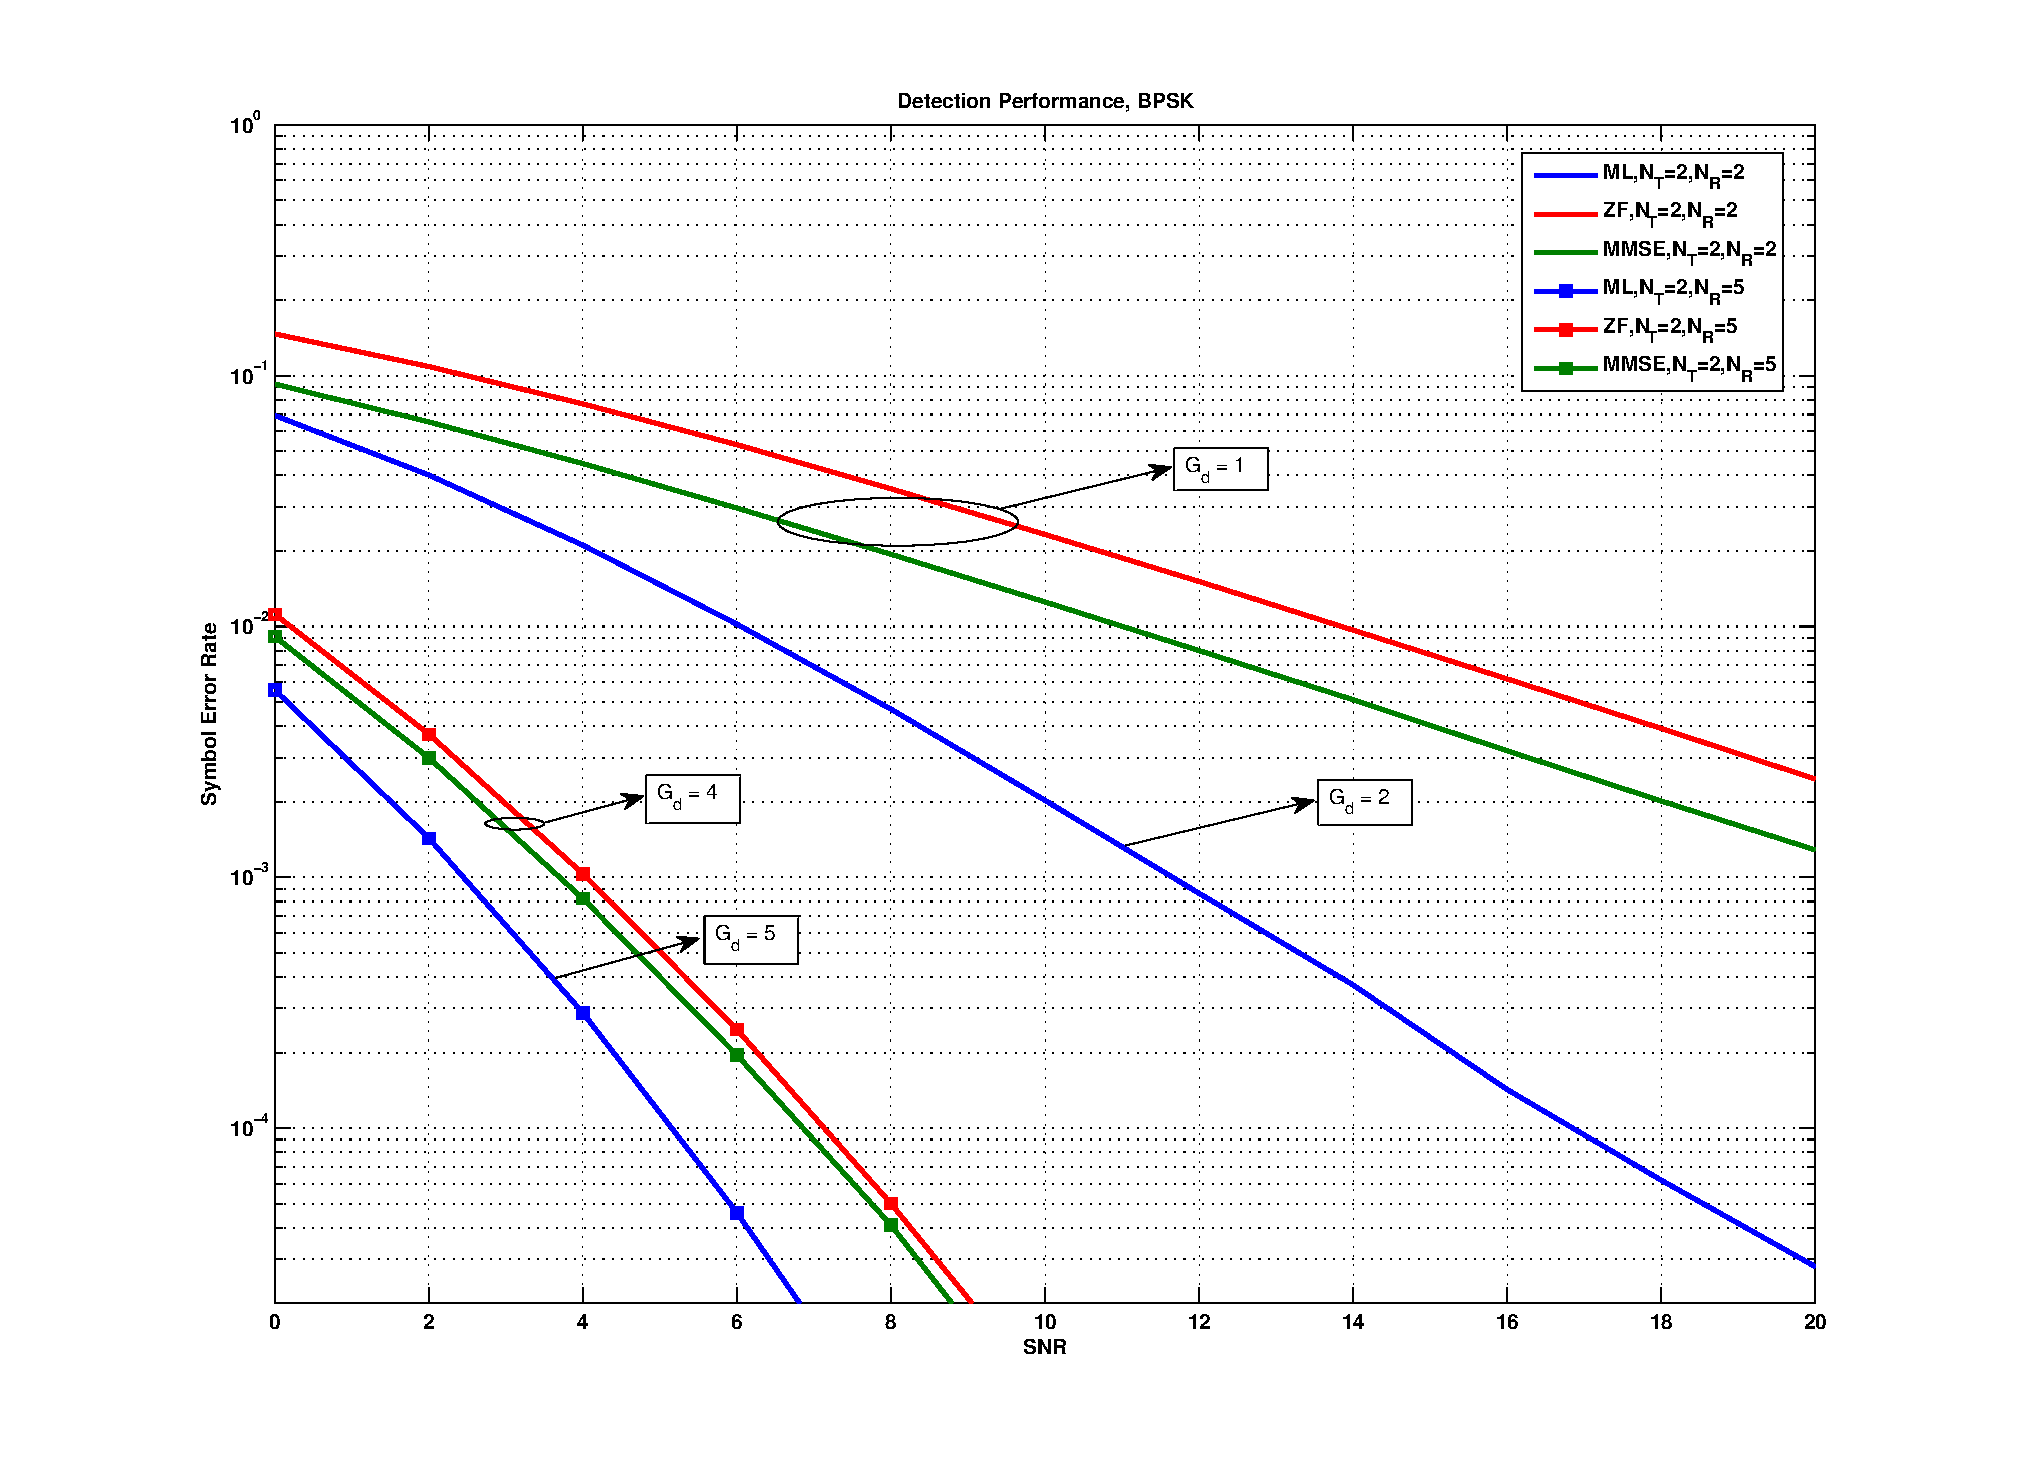
\includegraphics[width = \textwidth]{MMSE}
		\caption{MMSE}
		\label{fig:MMSE}
	\end{figure}
	
\paragraph{SNR (biased vs. unbiased)}
\paragraph{a) biased SNR}
\begin{align*}
	\text{SNR}_{\text{bias,m}} &= \frac{\mathcal{E}_s}{[\boldsymbol{\Phi}_{ee}]_{mm}} = \frac{\mathcal{E}_s}{\mathcal{E}_s(1 - K_{mm})} = \frac{1}{1 - K_{mm}}, \quad 1\leq m \leq 4 
\end{align*}
	\textit{Anmerkung: } $\mathbf{K} = \mathbf{F}_{\text{opt}}\cdot\mathbf{H} \rightarrow \text{SNR} = 1 $ \textit{falls } $ \mathbf{K} = \text{zeros()} \Rightarrow \text{woher SNR } = 1 $ \textit{ bei keiner Uebertragung?} $\Rightarrow $ \textit{ nicht vorteilhaft: siehe: b) unbiased SNR}  % \ref{unbiased_SNR}
but: 
\begin{itemize}
	\item $\text{SNR}_{\text{bias,m}} $ does not represent the actual SNR since the main diagonal elements of $ \mathbf{K} $ are smaller than 1
	\item $ \mathbf{r} = \mathbf{FHx} + \mathbf{Fn} = \mathbf{Kx} + \underbrace{\mathbf{F}\mathbf{n} }_{\mathbf{\tilde{n}} = [\tilde{n}_1, \dots,\tilde{n}_{N_T}]^T } $
	\item $r_m = \underbrace{K_{mm}}_{<1}x_m + \underset{ n\neq m}{\sum\limits^{N_T}_{n = 1}}K_{mn}x_n + \tilde{n}_m $
\end{itemize}
\paragraph{b) unbiased SNR}
\label{par:unbiased_SNR}
\begin{itemize}
	\item remove bias: $r_m^\prime = \dfrac{r_m}{K_{mm}} = x_m + \underbrace{\dfrac{\tilde{e}_m}{K_{mm}}}_{e^\prime_m} $
	\item SNR?
	\item scaling matrix: $ \mathbf{C} = \text{diag}\bigl\{\frac{1}{K_{11}}, \frac{1}{K_{22}}, \dots, \frac{1}{K_{N_TN_T}}  \bigr\} $
	\item $\mathbf{r}^\prime = \mathbf{Cr} \rightarrow \mathbf{e}^\prime = [e^\prime_1, \dots, e^\prime_{N_T}]^T = \mathbf{r}^\prime - \mathbf{x}  = \mathbf{Cr} - \mathbf{x} = \mathbf{CFy} - \mathbf{x} $
	\item $\boldsymbol{\Phi}_{e^\prime e^\prime} = \mathcal{E}\Bigl\{\bigr(\mathbf{CFy} - \mathbf{x}\bigr)\bigl(\mathbf{CFy} - \mathbf{x}\bigr)^H\Bigr\} = \mathbf{CF}\boldsymbol{\Phi}_{yy}\mathbf{F}^H\mathbf{C}^H - \mathbf{CF}\boldsymbol{\Phi}_{yx} - \boldsymbol{\Phi}_{xy}\mathbf{F}^H\mathbf{C}^H + \boldsymbol{\Phi}_{xx}$
	\item $ \mathbf{F} = 	\mathbf{F}_{\text{opt}} \rightarrow \mathbf{F}_{\text{opt}}\boldsymbol{\Phi}_{yy} = \boldsymbol{\Phi}_{xy} = \mathcal{E}_s\cdot\mathbf{H}^H $
	\item[$\rightarrow$] $\boldsymbol{\Phi}_{e^\prime e^\prime} = \mathcal{E}_s\mathbf{C}\underbrace{\mathbf{H}^H\mathbf{F}^H}_{\mathbf{K}^H}\mathbf{C}^H - \mathcal{E}_s\mathbf{C}\underbrace{\mathbf{FH}}_{\mathbf{K}} - \mathcal{E}_s\underbrace{\mathbf{H}^H\mathbf{F}^H}_{\mathbf{K}^H}\mathbf{C}^H  + \mathcal{E}_s\mathbf{I} \\ \quad = \mathcal{E}_s\bigl[\mathbf{I} + (\mathbf{C} - \mathbf{I})\mathbf{K}^H\mathbf{C}^H - \mathbf{CK}\bigr]$  
	\item[] \textit{Anmerkung: nur Hauptdiagonalelemente interessieren, da diese die Varianz darstellen}
	\item[$\rightarrow$] maindiagonal elements of $\boldsymbol{\Phi}_{e^\prime e^\prime} =  $ variances of $ e^\prime _m \quad = \mathcal{E}_s\Bigl ( 1 + \bigl (\frac{1}{K_{mm}} - 1\bigr )   K_{mm}\frac{1}{K_{mm}}  - \frac{1}{K_{mm}}  K_{mm}\Bigr )  = 
	\frac{1 - K_{mm}}{K_{mm}}$
	\item[$\rightarrow$] vgl. Abbildung \ref{MMSE}
	\item[$\rightarrow$]$SNR_{unbiased}=\dfrac{\mathcal{E}_s}{[\boldsymbol{\Phi}_{e^\prime e^\prime}]_{mm}}=\dfrac{\mathcal{E}_s}{\mathcal{E}_s\dfrac{1-K_{mm}}{K_{mm}}}
	=\dfrac{K_{mm}}{1-K_{mm}} = \frac{1}{1 - K_{mm}} - 1 = SNR_{biased} - 1, \quad 1\leq m \leq N_T$
	\item[$\rightarrow$]the SNR after bias removal is by ``$1$'' smaller than the biased SNR $\rightarrow$ general result valid for any type of
	MMSE estimation
\end{itemize}
\subsubsection{Decision\,-\,Feadback Equalization (Detection)}
\begin{itemize}
	\item Also known as: 
	\begin{itemize}
		\item BLAST (Bell Laboratories space-time system)
		\item successive interference cancellation		
	\end{itemize}
	\item Problem of linear receiver: Noise enhancementbecause of linear filtering $\rightarrow$ nonlinear filtering processing necessary
\end{itemize}
\paragraph{Basic Idea}
\begin{itemize}
	\item Recall (linear filter): $\mathbf{FH} = \mathbf{I} $ for linear ZF receiver $\rightarrow$ $i$th row of $\mathbf{F}, \mathbf{f}_i, $ is orthogonal to the $j$th column of $\mathbf{H}, \mathbf{h}_j$, if $ i \neq j$ (if $i = j$: inner product = 1)  
	\item we can detect $x_i$, based on $r_i = \mathbf{f}_i\mathbf{y} $
	\item Once we have detected $x_i$, we can substract its contribution from $\mathbf{y}$: $\mathbf{y}_1 = \mathbf{y} - \mathbf{h}_i\hat{x}_i$ ($\hat{x}_i $ is detected symbol, we assume for now, $\hat{x}_i = x_i $) 
	\item $\mathbf{y}_1 $ can be expressed as $ \mathbf{y}_1 = \mathbf{H}_i\mathbf{x}_i + \mathbf{n}$ where 
	\begin{align*}
		\mathbf{H}_i &= \bigl[\mathbf{h}_1, \dots ,\mathbf{h}_{i-1},\mathbf{h}_{i+1},\dots ,\mathbf{h}_{N_T} \bigr] \\
		\mathbf{x}_i &= \bigl[x_1, \dots , x_{i-1}, x_{i+1}, \dots ,x_{N_T}\bigr]
	\end{align*}
	\begin{itemize}
		\item[$\rightarrow$] we have reduced the number of signal streams to $N_T - 1$ ($N_R $ bleibt gleich)
	\end{itemize}
	\item apply now linear ZF filter for symbol to detected next, e.g. $x_j $, where $ j\in \bigl\{1, \dots ,i - 1, i + 1, \dots , N_T\bigr\} $
	\item[$\rightarrow$] $ \mathbf{r}_j = \mathbf{f}_j\mathbf{y}_1 $ where $\mathbf{f}_j $ is the ZF filter for $\mathbf{H}_1$ 
	\item substract contribution of $x_j $ from $\mathbf{y}_1 $: $\mathbf{y}_2 = \mathbf{y}_1 - \mathbf{h}_j x_j $
	\item substract until last symbol is detected
	\item Blockdiagram see figure\ref{DFE} 
	\begin{figure}[h]
		\centering
		\resizebox{\textwidth}{!}{\input{DFE.pstex_t}}
		\caption{DFE Blockdiagram}
		\label{fig:DFE.pstex_t}
	\end{figure}
	\item Observations:
	\begin{itemize}
		\item The order in which the $x_1 $ are detected can be freely chosen and effects the performance $\rightarrow  N_T! $ possible orders $\rightarrow$ cannot explore all of them
		\item Practical approach: Select in each step that $x_i $ for which the noise variance enhancement is minimum, i.e. which has the smallest $\mathcal{E}\Bigl\{|\mathbf{f}_i\mathbf{n}|^2\Bigr\} = \sigma _n^2\||\mathbf{f}_i\||^2 $ 
	\end{itemize}
	\item Diversity order:
	\begin{itemize}
		\item stage 1: $G_d^1 = N_R - N_T + 1 $
		\item stage 2: $G_d^2 = G_d^1 + 1 = N_R - N_T +2 $
		\item[ $\vdots$]
		\item stage $N_T$: $G_d^{N_T} = N_R $
		\item overall: $\underline{G_d = N_R - N_T +1} $
		\item \textit{(Anmerkung: der schlechteste Fall dominiert (Stage 1), weitere koennen nur schwer beeinflussen)}
	\end{itemize}
\end{itemize}
\paragraph{ZF - DFE - Matrix Model}
\begin{itemize}
	\item Signal model: $ \mathbf{y} = \mathbf{Hx} + \mathbf{n} = \underbrace{\mathbf{HP}}_{\tilde{\mathbf{H}}}\cdot\underbrace{\mathbf{P}^{-1}\mathbf{x}}_{\tilde{\mathbf{x}}} + \mathbf{n} $ with permutation matrix $\mathbf{P} $
	\item $\mathbf{P} $ has one \glqq 1\grqq\, per column and row, all other elements are \glqq 0\grqq 
	\item[$\rightarrow$] can change the detection order to maximize performance
	\item note: $\mathbf{P}^T = \mathbf{P}^{-1} $
	\item Example: 
	\begin{align*}
		\mathbf{P} &= \begin{pmatrix*}[r] 0 & 0 & 1\\1 & 0 & 0\\ 0 & 1 & 0	\end{pmatrix*}[r] \rightarrow \mathbf{P}^{-1} = \mathbf{P}^T = \begin{pmatrix*}0 & 1 & 0\\0 & 0 & 1\\ 1 & 0 & 0\end{pmatrix*}\\
		\tilde{\mathbf{x}} &= \mathbf{P}^T\cdot\mathbf{x} = \begin{pmatrix*}[r] 0 & 1 & 0\\ 0 & 0 & 1\\ 1 & 0 & 0\end{pmatrix*}\begin{pmatrix*}[r]x_1 \\x_2\\x_3\end{pmatrix*} = \begin{pmatrix*}[r]x_2\\x_3\\x_1\end{pmatrix*}
	\end{align*}
	\item Blockdiagram see figure \ref{ZF-DFE-Matrix}
	\begin{figure}
		\centering
		\resizebox{\textwidth}{!}{\input{ZF_DFE_Matrix.pstex_t}}
		\caption{ZF-DFE Matrix Model}
		\label{fig:ZF-DFE-Matrix_pstex_t}
	\end{figure}
	\item DFE Filters:
	\begin{itemize}
		\item $\mathbf{F}$ feedworward filter
		\item $\mathbf{B}$ feedback filter
	\end{itemize}
	\item Filter calculation
	\begin{itemize}
		\item Cholesky factorization: $\tilde{\mathbf{H}}^H \tilde{\mathbf{H}} = \mathbf{L}^H\mathbf{DL}$ with diagonal matrix $\mathbf{D}$
			and lower triangular matrix $\mathbf{L}$ ( maindiagonal elements of $\mathbf{L}$ are ``1'')
	\begin{align*}
			\mathbf{L} &= 
			\begin{bmatrix}
				1 & 0 & \cdots & \cdots & 0 \\
				l_{21} & 1 & \ddots & \ddots &	\vdots \\
				l_{31} & l_{32} & 1 & \ddots &\vdots \\
				\vdots & \ddots & \ddots & \ddots & \vdots\\
				\vdots & \cdots & \cdots & \cdots & 1
			\end{bmatrix}
	\end{align*}

		\item $\mathbf{F}=\mathbf{D}^{-1}\mathbf{L}^{-H}\tilde{\mathbf{H}}^H$
		\begin{align*}
			\rightarrow \mathbf{r}=\mathbf{Fy}=\underbrace{\mathbf{D}^{-1}\mathbf{L}^{-H}\underbrace{\tilde{\mathbf{H}}^H\tilde{\mathbf{H}}}_
			{\mathbf{L}^H\mathbf{DL}}}_{\mathbf{L}}\tilde{\mathbf{x}}+\underbrace{\mathbf{D}^{-1}\mathbf{L}^{-H}\tilde{\mathbf{H}}^H\mathbf{n}}_
			{\tilde{\mathbf{n}}}
		\end{align*}
		\item $\mathbf{B}=\mathbf{L-I}=$ lower triangular matrix with maindiagonal elements ``$0$''
	\begin{align*}
			\mathbf{B} &= 
			\begin{bmatrix}
				0 & 0 & \cdots & \cdots & 0 \\
				l_{21} & 0 & \ddots & \ddots &	\vdots \\
				l_{31} & l_{32} & 0 & \ddots &\vdots \\
				\vdots & \ddots & \ddots & \ddots & \vdots\\
				\vdots & \cdots & \cdots & \cdots & 0
			\end{bmatrix}
	\end{align*}

	\end{itemize}
	\item Interpretation:
	\begin{itemize}
		\item after feedforward filter
	\begin{align*}
			\mathbf{r} &= 
			\begin{bmatrix}
				1 & 0 & \cdots & \cdots & 0 \\
				l_{21} & 1 & \ddots & \ddots &	\vdots \\
				l_{31} & l_{32} & 1 & \ddots &\vdots \\
				\vdots & \ddots & \ddots & \ddots & \vdots\\
				\vdots & \cdots & \cdots & \cdots & 1
			\end{bmatrix}
			\begin{bmatrix}
				\tilde{x}_1 \\
				\tilde{x}_2 \\
				\vdots \\
				\tilde{x}_{N_T}
			\end{bmatrix}
			+ \tilde{\mathbf{n}}
	\end{align*}
	\end{itemize}
	\item from feedback filter
	\begin{align*}
			\tilde{\mathbf{r}} &= 
			\begin{bmatrix}
				0 & 0 & \cdots & \cdots & 0 \\
				l_{21} & 0 & \ddots & \ddots &	\vdots \\
				l_{31} & l_{32} & 0 & \ddots &\vdots \\
				\vdots & \ddots & \ddots & \ddots & \vdots\\
				\vdots & \cdots & \cdots & \cdots & 0
			\end{bmatrix}
			\begin{bmatrix}
				\hat{\tilde{x}}_1 \\
				\hat{\tilde{x}}_2 \\
				\vdots \\
				\hat{\tilde{x}}_{N_T}
			\end{bmatrix}
			\text{ $\hat{\tilde{x}}_n$ : decision on $\tilde{x}_n$}\\
			\rightarrow \mathbf{r}-\tilde{\mathbf{r}} &= 
			\begin{bmatrix}
			\tilde{x}_1+0 \\
			l_{21}(\tilde{x}_1-\hat{\tilde{x}}_1)+\tilde{x}_2+0 \\
			l_{31}(\tilde{x}_1-\hat{\tilde{x}}_2)+l_{32}(\tilde{x}_2-\hat{\tilde{x}}_2)+\tilde{x}_3+0 \\
			\vdots
			\end{bmatrix}
			+\tilde{\mathbf{n}}
	\end{align*}
\end{itemize}

\paragraph{MMSE-DFE}
\begin{figure}[h]
	\centering
	\input{MMSE_DFE.pstex_t}
	\caption{MMSE-DFE Blockdiagram}
	\label{fig:MMSE_DFE.pstex_t}
\end{figure}
\begin{itemize}
	\item $\mathbf{B}=\mathbf{L}-\mathbf{I}$ has to be lower triangular matrx with all-zero main diagonal elements because of causality.
	\item $\mathbf{d}=\mathbf{Fy}-\mathbf{B}\hat{\tilde{\mathbf{x}}} \quad \rightarrow \mathbf{e}=\mathbf{d}-\tilde{\mathbf{x}}=\mathbf{Fy}-\underbrace{(\mathbf{B}+\mathbf{I})}_{\mathbf{L}}\tilde{\mathbf{x}}$\\
	where we assume $\hat{\tilde{\mathbf{x}}}=\tilde{\mathbf{x}}$ for filter optimization
	\item Optimal $\mathbf{F}$ for given $\mathbf{L}$ \\
	\begin{align*}
		\sigma_e^2=\mathrm{tr}\left\{\underbrace{\mathcal{E}\{\mathbf{ee}^H\} }_{\boldsymbol{\Phi}_{ee}}\right\}
		=\mathrm{tr}\left\{\mathbf{F}\boldsymbol{\Phi}_{yy}\mathbf{F}^H\right\}-\mathrm{tr}\left\{\mathbf{F}\boldsymbol{\Phi}_{y \tilde{x}}\mathbf{L}^H\right\}
		-\mathrm{tr}\left\{\mathbf{L}\boldsymbol{\Phi}_{\tilde{x} y}\mathbf{F}^H\right\}
		+\mathrm{tr}\left\{\mathbf{L}\boldsymbol{\Phi}_{\tilde{x} \tilde{x}}\mathbf{L}^H\right\}
	\end{align*}
	\begin{align*}
		\dfrac{\delta}{\delta \mathbf{F}^*}\sigma_e^2=\mathbf{F}\boldsymbol{\Phi}_{yy}-\mathbf{L}\boldsymbol{\Phi}_{\tilde{x}y}=0 \quad \rightarrow \mathbf{F}
		=\mathbf{L}\boldsymbol{\Phi}_{\tilde{x}y}\boldsymbol{\Phi}_{yy}^{-1}
	\end{align*}
	where
	\begin{align*}
		\boldsymbol{\Phi}_{yy}&=\mathcal{E}_s\tilde{\mathbf{H}}\tilde{\mathbf{H}}^H+\sigma_n^2\mathbf{I}\\
		\boldsymbol{\Phi}_{\tilde{x}y}&=\mathcal{E}_s\tilde{\mathbf{H}}^H
	\end{align*}
	\begin{align*}
		\rightarrow \mathbf{F}=\mathbf{L}\tilde{\mathbf{H}}^H(\tilde{\mathbf{H}}\tilde{\mathbf{H}}^H + \dfrac{\sigma_n^2}{\mathcal{E}_s}\mathbf{I})^{-1}
		=\mathbf{L}\overbrace{(\tilde{\mathbf{H}}^H\tilde{\mathbf{H}}+\dfrac{\sigma_n^2}{\mathcal{E}_s}\mathbf{I})^{-1}\tilde{\mathbf{H}}^H}^{\text{MMSE Linear Equalizer}}
	\end{align*}
	\begin{figure}[h]
		\centering
		\resizebox{\textwidth}{!}{\input{DFE_MMSE_EQUIV.pstex_t}}
		\caption{MMSE-DFE Equivalence}
		\label{fig:MMSE_DFE_Equiv.pstex_t}
	\end{figure}
	\item Optimal $\mathbf{L}$:
	\begin{align*}
		\boldsymbol{\Phi}_{ee}&=\mathbf{L}\boldsymbol{\Phi}_{\tilde{x}y}\boldsymbol{\Phi}_{yy}^{-1}\boldsymbol{\Phi}_{yy}\boldsymbol{\Phi}_{yy}^{-1}\boldsymbol{\Phi}_{\tilde{x}y}^H\mathbf{L}^H
		-\mathbf{L}\boldsymbol{\Phi}_{\tilde{x}y}\boldsymbol{\Phi}_{yy}^{-1}\boldsymbol{\Phi}_{y\tilde{x}}\mathbf{L}^H
		-\mathbf{L}\boldsymbol{\Phi}_{\tilde{x}y}\boldsymbol{\Phi}_{yy}^{-1}\boldsymbol{\Phi}_{\tilde{x}y}^H\mathbf{H}^H+\mathbf{L}\boldsymbol{\Phi}_{\tilde{x}\tilde{x}}\mathbf{L}^H\\ 
		&=\mathbf{L}(\boldsymbol{\Phi}_{\tilde{x}\tilde{x}}-\boldsymbol{\Phi}_{\tilde{x}y}\boldsymbol{\Phi}_{yy}^{-1}\boldsymbol{\Phi}_{\tilde{x}y}^H)\mathbf{L}^H
	\end{align*}
	$=$ MMSE covariance matrix for a linear MMSE filter
	\begin{itemize}
		\item[$\rightarrow$]$\boldsymbol{\Phi}_{ee}=\sigma_n^2\mathbf{L}(\tilde{\mathbf{H}}^H\tilde{\mathbf{H}}+\dfrac{\sigma_n^2}{\mathcal{E}_s}\mathbf{I})^{-1}\mathbf{L}^H$
		\item[$\rightarrow$] need lower triangular matrix $\mathbf{L}$ which minimizes $\mathrm{tr}\{\boldsymbol{\Phi}_{ee}\}$
		\item[$\rightarrow$] the optimum $\mathbf{L}$ whitenes $\boldsymbol{\Phi}_{ee}$ $\rightarrow$  $\boldsymbol{\Phi}_{ee}$ becomes diagonal matrix,\\ i.e. $\mathbf{L}$ exploits the correlation after linear MMSE filtering to reduce noise variance!
		\item[$\rightarrow$] $\mathbf{L}$ is obtained via Cholesky factorization
		\begin{align*}
			\tilde{\mathbf{H}}^H\tilde{\mathbf{H}}+\dfrac{\sigma_n^2}{\mathcal{E}_s}\mathbf{I}=\mathbf{LDL}^H
		\end{align*}
		\item[$\rightarrow$] $\boldsymbol{\Phi}_{ee}=\sigma_n^2 \mathbf{L}(\mathbf{LDL}^H)^{-1}\mathbf{L}=\sigma_n^2\mathbf{LL}^{-1}\mathbf{D}^{-1}\mathbf{L}^{-H}\mathbf{L}^H=\sigma_n^2\mathbf{D}^{-1}\mathrel{\widehat{=}}$ diagonal matrix
	\end{itemize}
	\item Summary of MMSE calculation
	\begin{itemize}
		\item $\mathbf{B}=\mathbf{L}-\mathbf{I}$ where $\tilde{\mathbf{H}}^H\tilde{\mathbf{H}}+\dfrac{\sigma_n^2}{\mathcal{E}_s}\mathbf{I}=\mathbf{LDL}^H$
		\item $\mathbf{F}=\mathbf{L} \underbrace{(\tilde{\mathbf{H}}^H\tilde{\mathbf{H}}+\dfrac{\sigma_n^2}{\mathcal{E}_s}\mathbf{I})^{-1}\tilde{\mathbf{H}}^H}_{\mathbf{F}_{Linear}}$
		\item $\mathbf{L}$ is a prediction error filter, which whitenes the error signal $\mathbf{e}$
		\item SNR:
		\begin{align*}
			\mathbf{D}&=\mathrm{diag}\{\xi_1,\dots,\xi_{N_T}\}\\
			\boldsymbol{\Phi}_{ee}&=\mathrm{diag}\{\dfrac{\sigma_n^2}{\xi_1},\dots,\dfrac{\sigma_n^2}{\xi_{N_T}}\}
		\end{align*}
		\item end-to-end channel
		\begin{align*}
			\mathbf{K}&=\mathbf{F}\tilde{\mathbf{H}}\\
				&=\underbrace{\mathbf{L}(\tilde{\mathbf{H}}^H \tilde{\mathbf{H}}+ \dfrac{\sigma_n^2}{\mathcal{E}_s}\mathbf{I})^{-1}\mathbf{L}^H}_{\dfrac{1}{\sigma_n^2}\boldsymbol{\Phi}_{ee}} 
				\mathbf{L}^{-H} \tilde{\mathbf{H}}^H\tilde{\mathbf{H}}\\
				&= \dfrac{1}{\sigma_n^2} \boldsymbol{\Phi}_{ee} \mathbf{L}^{-H}(\tilde{\mathbf{H}}^H\tilde{\mathbf{H}}+\dfrac{\sigma_n^2}{\mathcal{E}_s}\mathbf{I}-\dfrac{\sigma_n^2}{\mathcal{E}_s}\mathbf{I})
				\mathbf{L}^{-1}\mathbf{L}\\
				&= \dfrac{1}{\sigma_n^2}\boldsymbol{\Phi}_{ee}[\underbrace{\mathbf{L}^{-H}(\tilde{\mathbf{H}}^H\tilde{\mathbf{H}}+\dfrac{\sigma_n^2}{\mathcal{E}_s}\mathbf{I})\mathbf{L}^{-1}}_{\sigma_n^2\boldsymbol{\Phi}_{ee}^{-1}}
				\mathbf{L}-\dfrac{\sigma_n^2}{\mathcal{E}_s}\mathbf{L}^{-H}]\\
				&=\mathbf{L}-\dfrac{1}{\mathcal{E}_s}\boldsymbol{\Phi}_{ee}\mathbf{L}^{-H}
		\end{align*}
		$\rightarrow$ main diagonal of $\mathbf{K}$:
		\begin{align*}
			K_{mm}=1-\dfrac{\sigma_n^2}{\mathcal{E}_s\xi_m} < 1
		\end{align*}
		\item biased SNR
		\begin{align*}
			SNR_{m,bias}=\dfrac{\mathcal{E}_S}{[\boldsymbol{\Phi}_{ee}]_{mm}}=\dfrac{\mathcal{E}_s}{\sigma_n^2}\xi_m=\dfrac{1}{1-K_{mm}}, \quad 1 \leq m \leq N_T
		\end{align*}
		\item unbiased SNR
		\begin{align*}
			SNR_{m,unbiased}=SNR_{m,bias}-1=\dfrac{1}{1-K_{mm}}-1=\dfrac{K_{mm}}{1-K_{mm}}, \quad 1 \leq m \leq N_T
		\end{align*}
	\end{itemize}
\end{itemize}

\subsubsection{Sphere Decoding}

\begin{itemize}
	\item Linear and DFE receivers cannot approach performance of ML\,-\,detector
	\item ML\,-\,detector: $ \hat{\mathbf{x}} = \underset{\mathbf{x} \in A^{N_T}}{\text{argmin}}||\mathbf{y} - \mathbf{Hx}||^2 $
	\item[$\rightarrow$] high complexity for brute force search
\end{itemize}
\paragraph{Main Idea}
\begin{itemize}
	\item can we search ML metric in a ``smarter'' way, akin to the smart search of the viterbi algorithm for problems with a trellis structure
	\item we need to find a way to prune/dismiss non\,-\,ML sequences/vectores early on
	\item[$\rightarrow$] this is accomplished by \underline{sphere decoding}	
\end{itemize}
\paragraph{Step 1}
Bring metric into a suitable form:
\begin{itemize}
	\item real represantation: $||\mathbf{y} - \mathbf{Hx}||^2 = ||\tilde{\mathbf{y}} - \tilde{\mathbf{H}}\tilde{\mathbf{x}}||^2 $
	\item where:
	\begin{align*}
		\tilde{\mathbf{y}} &= \begin{bmatrix*} \operatorname{Re}\{\mathbf{y}^T\} & \operatorname{Im}\{\mathbf{y}^T \}	\end{bmatrix*}^T \\
		\tilde{\mathbf{x}} &= \begin{bmatrix*} \operatorname{Re}\{\mathbf{x}^T\} & \operatorname{Im}\{\mathbf{x}^T \}	\end{bmatrix*}^T \\
		\tilde{\mathbf{H}} &= \begin{bmatrix*}[r] \operatorname{Re}\{\mathbf{H}\} & -\operatorname{Im}\{\mathbf{H} \} \\ \operatorname{Im}\{ \mathbf{H}\} &\operatorname{Re}\{\mathbf{H} \}\end{bmatrix*}^T 		
	\end{align*}
	\item[$\rightarrow$] QAM: $\tilde{\mathbf{x}}$ defines points in an $ 2N_T $ dimensional lattice
	\item QL decomposition: $ \tilde{\mathbf{H}} = \mathbf{QL} $ with
	\begin{itemize}
		\item orthogonal matrix $\mathbf{Q} \in\mathbb{R} ^{2N_T\times 2N_T};\quad \mathbf{QQ}^T = \mathbf{I}$ 
		\item and lower triangular matrix $\mathbf{L} \in \mathbb{R} ^{2N_T\times2N_T}$	
	\end{itemize}
	\begin{align*}
		||\tilde{\mathbf{y}} - \mathbf{QL}\tilde{\mathbf{x}}||^2 &= 
		||\mathbf{QQ}^T(\tilde{\mathbf{y}} - \mathbf{QL}\tilde{\mathbf{x}})||^2 + ||(\mathbf{I} - \mathbf{QQ}^T)(\tilde{\mathbf{y}} - \mathbf{QL}\tilde{\mathbf{x}})||^2 \\ 
		&= ||\mathbf{Q}(\mathbf{Q}^T\tilde{\mathbf{y}} - \mathbf{L}\tilde{\mathbf{x}})||^2 + ||(\mathbf{I} - \mathbf{QQ}^T)\tilde{\mathbf{y}} - \underbrace{(\mathbf{Q} - \mathbf{Q})}_{ = 0}\mathbf{L}\tilde{\mathbf{x}}||^2 \\ &= ||\mathbf{Q}^T\tilde{\mathbf{y}} - \mathbf{L}\tilde{\mathbf{x}}||^2 + \underbrace{||(\mathbf{I} - \mathbf{QQ}^T)\tilde{\mathbf{y}}||^2}_{\text{unabh\"angig von }\tilde{\mathbf{x}}}
	\end{align*}		 
	\item[$\Rightarrow $] $ \underset{\tilde{\mathbf{x}} \in A^{2N_T}}{\text{argmin}} ||\tilde{\mathbf{y}} - \tilde{\mathbf{H}}\tilde{\mathbf{x}}||^2 = \underset{\tilde{\mathbf{x}} \in A^{2N_T}}{\text{argmin}} ||\underbrace{\mathbf{Q}^T\tilde{\mathbf{y}}}_{\bar{\mathbf{y}}} - \mathbf{L}\tilde{\mathbf{x}}||^2$\\
	 where $A^{2N_T} $ contains all $ M^{N_T} $ possible vectors $\tilde{\mathbf{x}}$
	\item Observation:
	\begin{itemize}
		\item with
		\begin{align*}
			\mathbf{L} &= 
			\begin{bmatrix}
				l_{11} & 0 & \cdots & 0 \\
				l_{21} & l_{22} & \ddots &	\vdots \\
				\vdots & & \ddots & 0\\
				l_{2N_T\,1} & \cdots & & l_{2N_T\,2N_T}
			\end{bmatrix}\\
			\bar{\mathbf{y}} &= 
			 \begin{bmatrix}
			 	\bar{y}_1 & \cdots	& \bar{y}_{2N_T}
			 \end{bmatrix}^T \, ;\quad	
			 \tilde{\mathbf{x}} =
			 \begin{bmatrix}
			 	\tilde{x}_1 & \cdots	 & \tilde{x}_{2N_T}
			 \end{bmatrix}		 
		\end{align*}
		\item we have 
		\begin{align}\label{eq:Sphere_Decoding_01}
			||\bar{\mathbf{y}} - \mathbf{L}\tilde{\mathbf{x}}||^2 = (\bar{y} - l_{11}\tilde{x}_1)^2 + (\bar{y}_2 - l_{21}\tilde{x}_1 - l_{22}\tilde{x}_2)^2 + (\bar{y}_3 - l_{31}\tilde{x}_1 - l_{32}\tilde{x}_2 - l_{33}\tilde{x}_3)^2 + \ldots
		\end{align}
		\end{itemize}
		\item[$\rightarrow$] the $n$-th term in the above sum contains only $ \tilde{x}_1, \tilde{x}_2, \ldots,\tilde{x}_n $
\end{itemize}
\paragraph{Step 2}
Sphere decoding algorithm\\ 
\underline{\textbf{Define:}}
\begin{align*}
	 d(\tilde{\mathbf{x}}) &= \sum_{n = 1}^{2N_T} f_n(\tilde{\mathbf{x}}_n) \ ;\quad \text{with}\ f_n(\tilde{\mathbf{x}}_n) = \bigl (\bar{y}_n - \sum_{i = 1}^{n}l_{ni}\tilde{x}_i\bigr)^2\ ;\quad \tilde{\mathbf{x}}_n = 
	 \begin{bmatrix}
	 	\tilde{x}_1 & \ldots & \tilde{x}_n
	 \end{bmatrix}^T \\
	 d_n(\tilde{x}_n) &= \sum_{m = 1}^{n} f_n(\tilde{\mathbf{x}}_m)
\end{align*}
\underline{\textbf{Main Idea:}}
\begin{itemize}
	\item Assume we know that $ d(\tilde{\mathbf{x}}) \leq R $ holds for some $\tilde{\mathbf{x}} $, where $ R $ is the so called ``sphere radius" \quad	$\rightarrow$ any $ \tilde{\mathbf{x}} $ with $ d(\tilde{\mathbf{x}}) \geq R $ cannot be the ML solution and can be discarded
	\item since $ d_{n + 1}(\tilde{\mathbf{x}}_n^\prime, \tilde{x}_{n + 1}) \geq d_n(\tilde{\mathbf{x}}_n^\prime) $, we can easily discard $ \mathbf{x}_n^\prime $ and all \\ possible $ \tilde{\mathbf{x}} = \begin{bmatrix}
	\tilde{\mathbf{x}}_n^{\prime} & \tilde{x}_{n+1} & \tilde{x}_{n+2} & \ldots & \tilde{x}_{2N_T} \end{bmatrix}^T $ if we find $ d_n(\tilde{\mathbf{x}}_n^\prime) > R \quad $ \\ $ \Rightarrow $ we can exclude many possible vectors $\tilde{\mathbf{x}} $ without evaluating  any metrics for them 
	\item How to find a suitable $R$?
	\begin{itemize}
		\item Initial $R$: $R = d(\tilde{\mathbf{x}}_{\text{subopt}}) $ where $ \tilde{\mathbf{x}}_{\text{subopt}} $ was obtained with some suboptimum receiver
		\item $R $ is updated as $ R = R_{\text{new}} = d(\tilde{\mathbf{x}}_{\text{cand}}) $ where $ \tilde{\mathbf{x}}_{\text{cand}} $ is an $ \tilde{\mathbf{x}} $ which \\ yields  $ d(\tilde{\mathbf{x}}_{\text{cand}}) < R_{\text{old}} = R $
	\end{itemize}
	\item Use tree structure to represent all possible $\tilde{\mathbf{x}} $ 
\end{itemize}
\subparagraph{Example:}	

% Optionen für Stil, der im Bild verwendet werden kann
% Verwendung: \node [baumnode]
%
%\tikzset{
% 	baumnode/.style = {fill = gray, circle,draw}
% } 
% 
%\newpage
\begin{figure}[h]

\scalebox{0.8}[0.8]{ 
\begin{tikzpicture}[->,>=stealth']
\tikzstyle{every node} = [font = \small]
	\node [circle , draw]  (Start) {Start} 
		child {node [ circle, draw] (links) {links}
			edge from parent
			node[left] {$-1$}				
		}
		child {node [ circle, draw] (rechts) {rechts}
			edge from parent
			node[right] {$+1$}				
		}
	;
\end{tikzpicture}
}
\begin{center}
\begin{tikzpicture}%[rotate = 90]
\tikzstyle{level 1}=[sibling distance = 77mm]
\tikzstyle{level 2}=[sibling distance = 40mm]
\tikzstyle{level 3}=[sibling distance = 20mm]
\tikzstyle{level 4}=[sibling distance = 10mm]
%\tikzstyle{level 5}=[sibling distance = 30mm]
\tikzstyle{every node} = [font = \small]
		\node [circle, draw] (0) {0}
			child {node [circle,draw] (1) {1}
				child {node (0) [circle,draw] (2) {2}
					child {node [circle,draw] (4) {4}
						child {node [circle,draw] (8) {8}
							edge from parent
							node[above ] {$f_4(\ldots) = 4$}
						}
						child {node [circle,draw] (9) {9}
							child[grow=down] {node (x_subopt) {$\hat{x}_{\text{subopt}} = [-1,-1,-1,+11]^T$} edge from parent[->,>=stealth']}					
	%						child[missing] {node (Platzhalter){Platzhalter}}
							edge from parent
							node[below ] {$f_4(\ldots) = 2$}						
						}	
						edge from parent
						node[above ] {$f_3(\ldots) = 2$}		
					}
					child {node [circle,draw] (5) {5}
						child {node [circle,draw] (10) {10}
%							child[missing] {node (Platzhalter){Platzhalter}}
%							child  {node (x_ML) {$\hat{x}_{\text{ML}} = [-1,-1,+1,-11]^T$} edge from parent[->,>=stealth']}	
							edge from parent
							node[above ] {$f_4(\ldots) = 1$}						
						}
						child {node [circle,draw] (11) {11}
							edge from parent
							node[below ] {$f_4(\ldots) = 3$}						
						}			
						edge from parent
						node[below ] {$f_3(\ldots) = 1$}				
					}
					edge from parent
					node[left ] {$	f_2(-1,-1) = 2$}
				}
				child {node [circle,draw] (3) {3}
					child {node [circle,draw] (6) {6}
						child {node [circle,draw] (12) {12}}
						child {node [circle,draw] (13) {13}}		
						edge from parent
						node[above] {$f_3(\ldots) = 6$}			
					}
					child {node [circle,draw] (7) {7}
						child {node [circle,draw] (14) {14}
							child[grow=down]  {node (x_ML) {$\hat{x}_{\text{ML}} = [-1,-1,+1,-11]^T$} edge from parent[draw=none] }									}
						child {node [circle,draw] (15) {15}}	
						edge from parent
						node[below] {$f_3(\ldots) = 7$}	
					}				
					edge from parent
					node[right ] {$f_2(-1,+1) = 1$}				
				}	
				edge from parent
				node[left ] {$	f_1(-1) = 1$}		
			}
			child {node [circle,draw] (16) {16}
				child {node [circle,draw] (17) {17}
					child {node [circle,draw] (19) {19}
						child {node [circle,draw] (23) {23}}
						child {node [circle,draw] (24) {24}}						
						}
					child {node [circle,draw] (20) {20}
						child {node [circle,draw] (25) {25}}
						child {node [circle,draw] (26) {26}}						
						}
					edge from parent
					node[above] {$f_2(+1,-1) = 4$}		
					}
				child {node [circle,draw] (18) {18}
					child {node [circle,draw] (21) {21}
						child {node [circle,draw] (27) {27}}
						child {node [circle,draw] (28) {28}}						
					}
					child {node [circle,draw] (22) {22}
						child {node [circle,draw] (29) {29}}
						child {node [circle,draw] (30) {30}}						
					}
					%child[grow=down] {node (Punkte) {$\vdots$} edge from parent[draw=none]}
					edge from parent
					node[below] {$f_2(+1,+1) = 3$}						
				}	
				edge from parent
				node[right] {$f_1(+1) = 5$}				
			}
			;
			\draw[->,>=stealth'] (10)--(x_ML)	;

\end{tikzpicture}
	\caption{$\text{BPSK} = 2,\ N_T = 2$}
	\label{fig:tikz_Sphere_Decoding}
\end{center}
\end{figure}



\begin{itemize}
	\item Siehe dazu Abbildung \ref{fig:tikz_Sphere_Decoding} auf S. \pageref{fig:tikz_Sphere_Decoding}
	\item Assume $\tilde{\mathbf{x}}_{\text{subopt}} = \begin{bmatrix} -1 & -1 & -1 & 1	\end{bmatrix}^T $ \\ $ \quad \Rightarrow d(\tilde{x}_{\text{subopt}} = 1 + 2 + 2 + 2 = 7 = R $
	\item For $\tilde{x}_1 = 1 $ we find $ d_2(1,1) = 5 + 3 = 8 > R $ and $ d(1,-1) = 5 + 4 > R $ \\ $ \quad\Rightarrow $ we don't have to calculate metrics for remaining branches, i.e., for nodes $19, \ldots ,31 $
	\item For $ \tilde{x}_1 = -1 $ and $ \tilde{x}_2 = 1$ , we find that $d_3(-1, 1, -1) = 8 > R $ and $ d_3(-1, 1, 1) = 9 > R$ \\ $ \quad\Rightarrow $ remaining branches emerging from nodes 6 and 7 can be discarded
	\item For the ML solution we find $d(-1, -1, 1, -1) = 5 < R $
	\item Different strategies exist, regarding in which order the nodes in the tree (points in the lattice) are investigated
	\begin{itemize}
		\item Pohst strategy
		\item Schnoir\,-\,Enchner strategy
		\item rich literature on lattice decoding algorithms
	\end{itemize}
	\item Complexity of sphere decoding
	\begin{itemize}
		\item worst-case complexity is still exponential in $N_T$
		\item (for practical case:) for sufficiently high SNR, the average complexity is only polynomial in $N_T \Rightarrow $ efficient ML decoding
	\end{itemize}		
	\item sphere decoding has found application in many fields:
	\begin{itemize}
		\item ML detection in MIMO and multiuser systems
		\item precoding
		\item source coding
		\item multiple symbol differential detection
	\end{itemize}
\end{itemize}


\end{document}
